
\section{Strategie di controllo errore}
I pacchetti di livello 2 sono chiamati frame/trame, sono divisi in header e trailer; nel trailer sono presenti i campi utili alle strategie di controllo degli errori.

È possibile distinguere due tipi principali di strategie:
\begin{enumerate}
    \item FEC (Forward Error Correction): il mittente invia dati ridondanti, in modo che il destinatario possa correggere gli errori senza richiedere una ritrasmissione.
    \item ARQ (Automatic Repeat-reQuest): il mittente invia i dati e il destinatario richiede la ritrasmissione dei dati corrotti. 
\end{enumerate}

\begin{figure}[htbp]
    \centering
    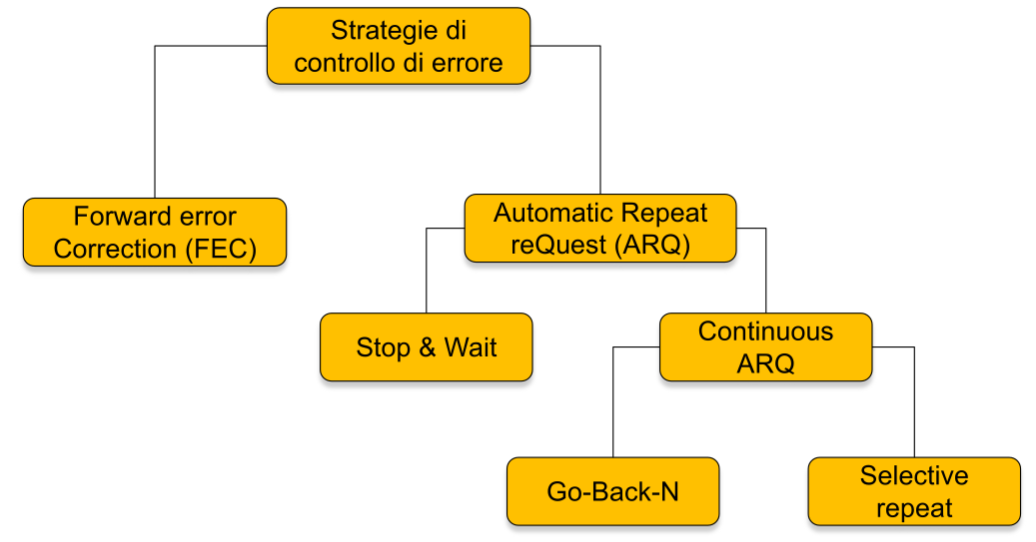
\includegraphics[width=0.7\textwidth]{images/strategierrore.png}
    \caption{Strategie di controllo degli errori: confronto tra FEC e ARQ}
\end{figure}

\subsection{Protocolli ARQ (Automatic Repeat-reQuest)}
Nei sistemi di telecomunicazioni, Automatic Repeat-reQuest è una strategia di controllo di errore, che svolge il compito di rivelare un errore (ma non di correggerlo). I pacchetti corrotti vengono scartati e viene richiesta la loro ritrasmissione.
I protocolli di tipo ARQ più comuni sono:

\begin{multicols}{3}
\begin{itemize}
    \item Stop-and-Wait 
    \item Go-Back-N 
    \item Selective Repeat
\end{itemize}
\end{multicols}


\newpage
\subsubsection{Stop-and-Wait}
Lo stop-and wait è un protocollo di tipologia Continous ARQ, per cui è ammessa la trasmissione continua di più frame numerati.

In questo caso specifico, i segnali di riscontro negativi sono cumulativi.

\begin{figure}[htbp]
    \centering
    \begin{minipage}{0.4\textwidth}
        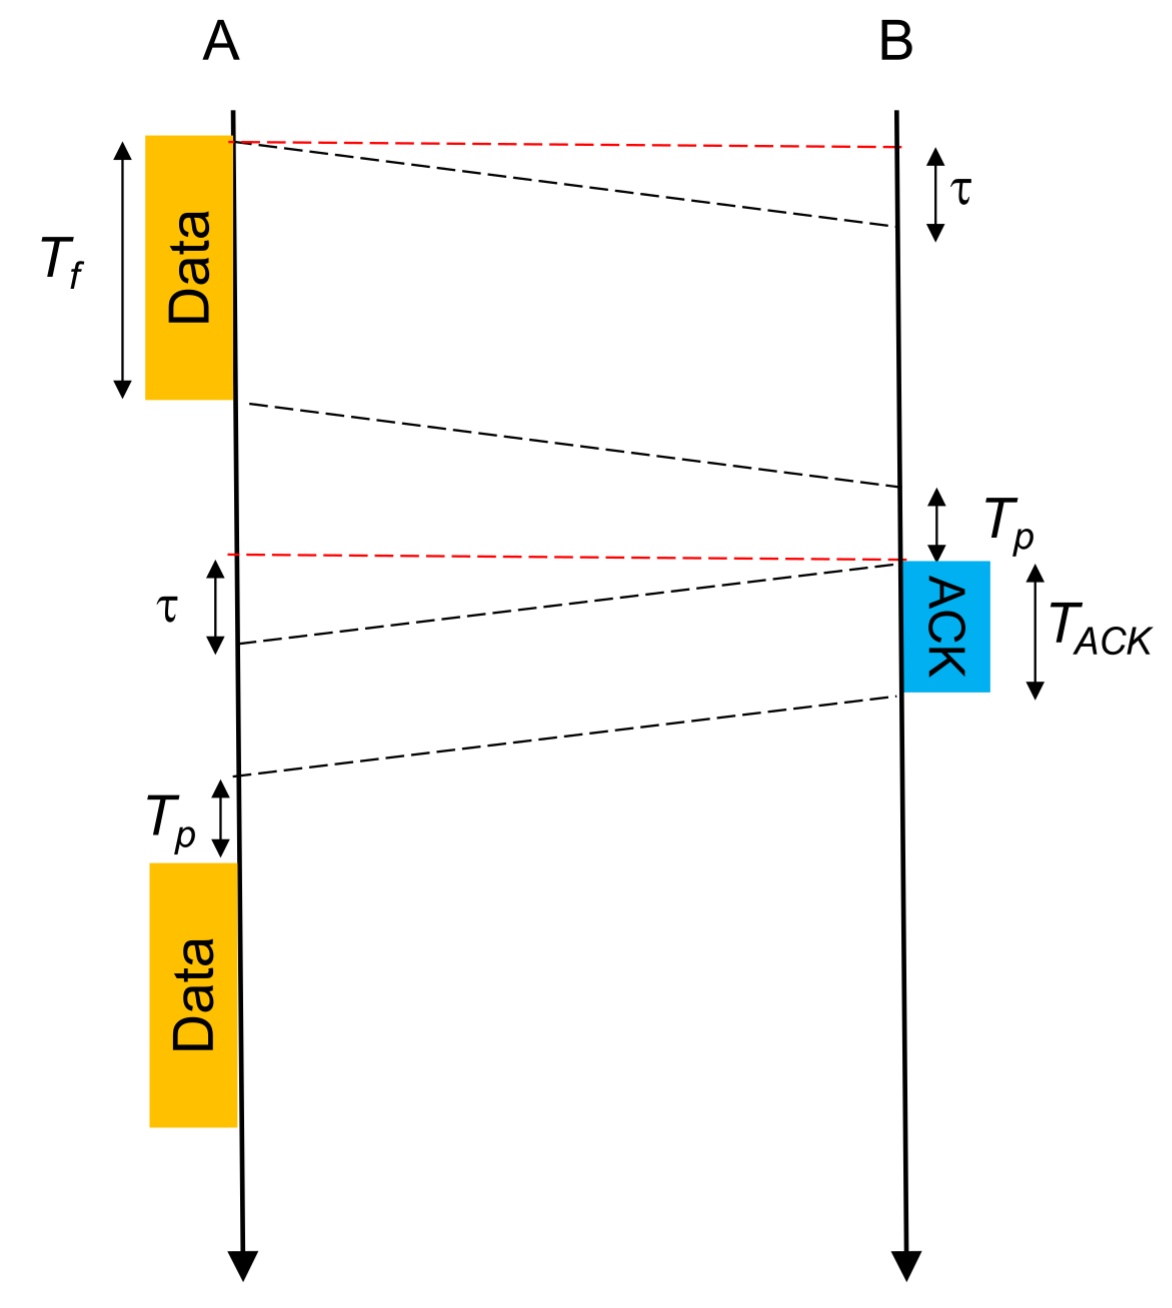
\includegraphics[width=\linewidth]{images/stopwait.png}
        \caption{Schema Stop-and-Wait}
    \end{minipage}%
    \hfill
    \begin{minipage}{0.55\textwidth}
        Il protocollo Stop-and-Wait prevede che il mittente attenda il riscontro del destinatario per ogni frame inviato, prima di procedere con il frame successivo.

        Il mittente invia una trama, quindi si ferma (stop) e attende (wait) il riscontro (Ack) da parte del ricevente prima di trasmettere una nuova trama.
\begin{itemize}
    \item $T_f$: tempo di trasmissione di una trama [s]
    \item $T_{ACK}$: tempo di trasmissione di un riscontro [s]
    \item $T_p$: tempo di elaborazione di una trama [s]
    \item $\tau$: tempo di propagazione [s]
\end{itemize}
    \end{minipage}
\end{figure}

\subsection{Efficienza di stop and wait in assenza di errori}

Prima di definire l'efficienza del protocollo, è necessario definire il tempo necessario a trasmettere una trama:

\begin{equation}
T_{tot} = T_f + T_{ACK} + 2T_p + 2\tau
\end{equation}

$T_p$ come già detto è il tempo di elaborazione della trama, dipende dalla valocità di elaborazione e quindi non dovrebbe essere precisamente uguale in trasmissione e ricezione, ma per semplicità lo consideriamo uguale.
Inoltre $T_f$, il tempo di trasmissione della trama, è anche definito come il tempo utile, poichè tutti gli altri tempi che consideriamo sono relativi a operazioni di controllo,elaborazione e invio del pacchetto
L'efficienza ($\eta$) è perciò definita come:
\begin{equation}
\eta = \frac{T_f}{T_{tot}} = \frac{T_f}{T_f + T_{ACK} + 2T_p + 2\tau}
\end{equation}

Si possono effettuare alcune semplificazioni, considerando che $T_{ACK}$ e $T_p$ sono molto più piccoli di $T_f$ e $\tau$, quindi possiamo considerare:

\begin{equation}
T_{tot} = T_f + 2\tau
\end{equation}
da cui si ottiene l'efficienza:

\begin{equation}
\eta = \frac{T_f}{T_f + 2\tau} = \frac{1}{1 + 2\frac{\tau}{T_f}} = \frac{1}{1 + 2\alpha} 
\end{equation}
dove $\alpha$ = $\frac{\tau}{T_f}$ è il rapporto di propagazione normalizzato

\begin{itemize}
    \item il throughput è pari al prodotto tra la frequenza di cifra C (capacità del canale) e l'efficienza: $\eta$C
    \item anche in assenza di errori, l'efficienza non è mai pari a 1.
\end{itemize}

\newpage

\subsection{Efficienza di stop and wait in presenza di errori}

I problemi che possono verificarsi sono:
\begin{multicols}{2}
\begin{itemize}
    \item il frame o l'ACK arrivano errati
    \item il frame non arriva
\end{itemize}
\end{multicols}

\begin{figure}[htbp]
    \centering
    \begin{minipage}{0.44\textwidth}
        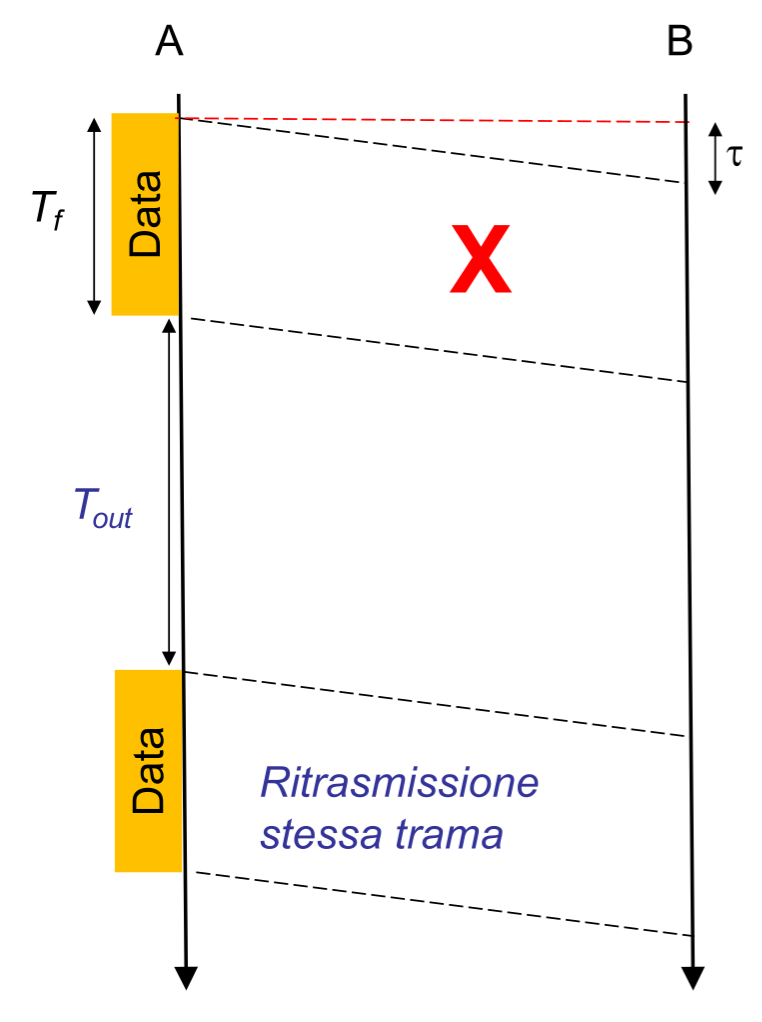
\includegraphics[width=\linewidth]{images/erroreframe.png}
        \caption{Errore nel frame: quando si verifica un errore nel frame, il mittente si accorge del problema grazie alla scadenza del timer avviato durante la trasmissione. 
        In tal caso, il frame viene ritrasmesso. Questo processo garantisce che i dati vengano ricevuti correttamente, ma può ridurre l'efficienza del protocollo a causa delle ritrasmissioni necessarie.}
    \end{minipage}%
    \hfill
    \begin{minipage}{0.48\textwidth}
        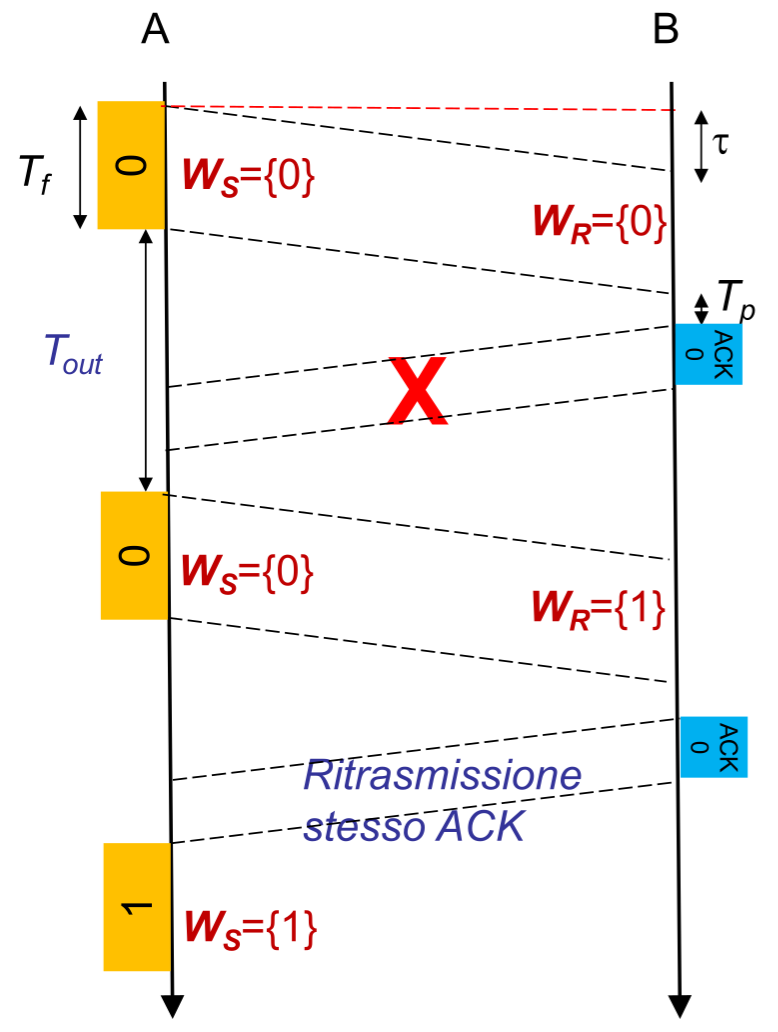
\includegraphics[width=\linewidth]{images/erroreack.png}
        \caption{Errore nell'ACK: quando si verifica un errore nell'ACK, il mittente non riceve il riscontro atteso entro il tempo stabilito dal timer. 
        Anche in questo caso, il frame viene ritrasmesso. }
    \end{minipage}
\end{figure}

Come calcolo il $T_{out}$(time che avvio nel momente nella trasmissione del frame)?

Deve valere almeno il tempo di invio del ACK($T_{ACK}$), più il tempo di propagazione(andata e ritorno) più il tempo di elaborazione del frame($T_p$, in ricezione e trasmissione):
\begin{equation}
T_{out} \geq T_{ACK} + 2\tau + 2T_p
\end{equation}

Il numero di frame ritrasmessi per la corretta ricezione del frame è detto $N_S$ ed è in media considerabile come una variabile aleatoria;

inoltre il numero totale di frame trasmessi($N_R$) è dato dal numero di frame ritrasmessi più il frame inviato con successo:
\begin{equation}
N_R = N_S + 1
\end{equation}

Per calcolare il tempo totale necessario per la trasmissione
si deve considerare che per ogni ritrasmissione si perde un
tempo pari a $T_f+T_{out}$ cui si deve aggiungere il tempo
necessario per la trasmissione che avviene con successo:
\begin{equation}
T_{tot} = (N_S - 1)(T_f + T_{out}) + T_f + T_{ACK} + 2T_P + 2\tau
\end{equation}
\newpage

\paragraph{Calcolo di $\overline{N_S}$}
la variabile $N_S$ è aleatoria, in quanto
dipende dagli errori sul canale di trasmissione; 
si calcola l'efficienza media del protocollo SW in presenza di errori considerando il valor
medio di $N_S$
\begin{figure}[htbp]
    \centering
    \begin{minipage}{0.45\textwidth}
        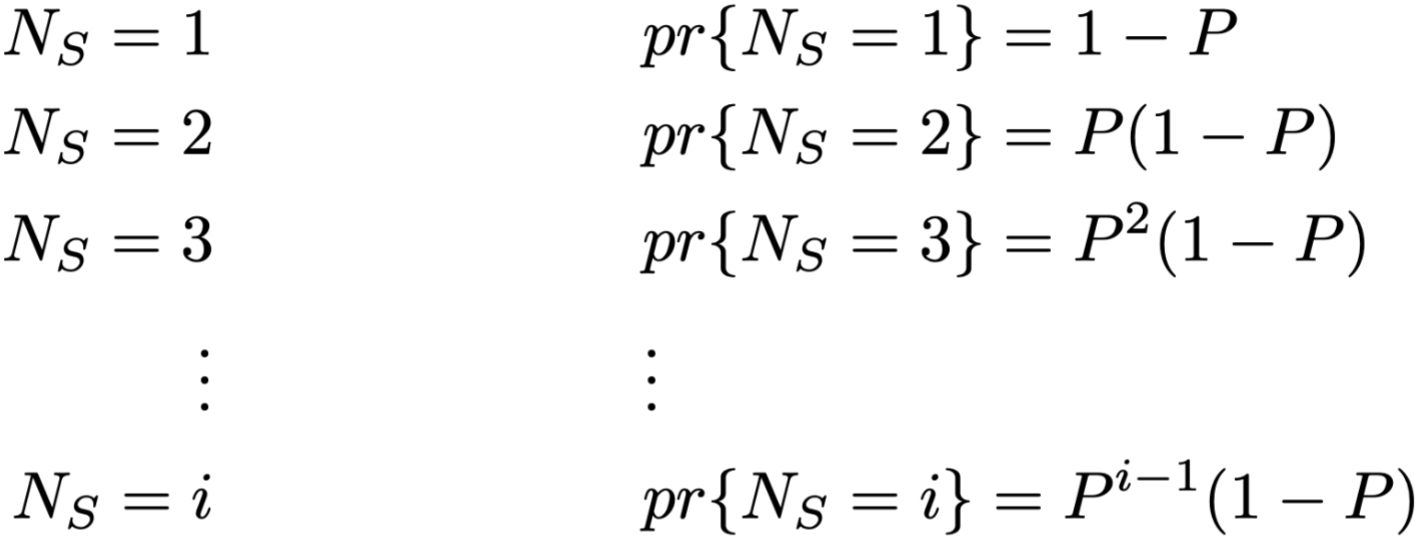
\includegraphics[width=\linewidth]{images/swprobabilita.png}
        \caption{Probabilità di successo e insuccesso nella trasmissione di un frame in Stop-and-Wait}
    \end{minipage}%
    \hfill
    \begin{minipage}{0.5\textwidth}
        Definiamo il frame error rate (FER) come la probabilità che un frame venga ricevuto con errore, che sarà il valore di P nel calcolo successivo. 
            Se $P$ è la probabilità che un frame sia errato, la probabilità che un frame sia trasmesso correttamente è $1-P$.
       
        La variabile aleatoria $N_S$ rappresenta il numero di tentativi necessari affinché un frame sia ricevuto correttamente. 
        
        La sua distribuzione è di tipo geometrico:
        \begin{equation*}
            P(N_S = k) = P^{i-1}(1-P)
        \end{equation*}
        dove $k$ è il numero di tentativi (ritrasmissioni più il primo invio).
        Il valor medio di $N_S$ è:
        \begin{equation*}
            \overline{N_S} = \frac{1}{1-P}
        \end{equation*}
    \end{minipage}
\end{figure}



\begin{equation*}
 \overline{N_S} = E[N_S] = \sum_{i=1}^{+\infty} i P^{i-1}(1-P) = \frac{1}{(1-P)^2}(1-P) = \frac{1}{1-P}
\end{equation*}

\paragraph{Spiegazione}
La formula sopra mostra il calcolo del valor medio $\overline{N_S}$ per una variabile aleatoria geometrica, che rappresenta il numero medio di tentativi necessari affinché un frame venga trasmesso correttamente. 

La distribuzione geometrica è appropriata perché ogni trasmissione è indipendente e la probabilità di successo (ricezione corretta) è costante e pari a $1-P$, dove $P$ è la probabilità di errore del frame. La somma $\sum_{i=1}^{+\infty} i P^{i-1}(1-P)$ rappresenta la media pesata di tutti i possibili numeri di tentativi, ciascuno moltiplicato per la probabilità che siano necessari esattamente $i$ tentativi. 

Sviluppando la somma, si ottiene che il valor medio è $\frac{1}{1-P}$: questo significa che, in media, il numero di tentativi cresce all'aumentare della probabilità di errore $P$. Se $P$ è vicino a zero, bastano pochi tentativi; se $P$ aumenta, il numero medio di ritrasmissioni cresce rapidamente.

Perciò, ripetendo, se si vuole ottenere il valore medio di una variabile aleatoria bisogna effettuare uno studio probabilistico; questa probabilità aleatoria sarà in media pari alla moltiplicazione tra due probabilità:
\begin{itemize}
    \item probabilità di successo (1-P): frame trasmesso correttamente
    \item $P^{i-1}$ rappresenta la sequenza di fallimenti che avvengono prima della trasmissione avvenuta con successo, che calcolo per un valore di i infinito(serie geometrica), caso peggiore(benchè irreale)
\end{itemize}


\[
\Pr(N_S = i) = \underbrace{P^{i-1}}_{\text{\# fallimenti}} \cdot \underbrace{(1 - P)}_{\text{successo finale}}
\]

La distribuzione di probabilità è:
\[
\Pr(N_S = i) = P^{i - 1} (1 - P)
\]

Il valore atteso si ottiene come:
\[
\mathrm{E}[N_S] = \sum_{i = 1}^{\infty} i \cdot \Pr(N_S = i)
\]

\newpage

\subsubsection{Errore sul bit ed errore sul frame}
\paragraph{Frame error rate (FER)} è possibile definire le probabilità per le quali ci sia un errore sui bit(BER, bit error rate) all'interno di un range oppure, di maggiore interesse a questo livello di rete, la probabilità di errore su un range di frame, quindi il FER(frame error rate).

Per calcolarlo ci interessa definire:
\begin{itemize}
    \item $L_f$: lunghezza in bit del frame
    \item $L_{ACK}$: lunghezza in bit del ACK
\end{itemize}

e sarà pari al valore P utilizzato nel calcolo probabilistico precedente, perciò: 
\begin{equation}
P = FER = 1 - (1 - p)^{(L_f + L_{ACK})}
\end{equation}
\subsubsection{Calcolo dell'efficienza}
L'efficienza $\eta$ del protocollo Stop and wait è data da:

L'efficienza $\eta$ del protocollo Stop-and-Wait in presenza di errori si calcola come rapporto tra il tempo utile di trasmissione e il tempo totale medio necessario per trasmettere correttamente un frame, considerando anche le ritrasmissioni dovute agli errori:

\begin{equation}
\eta = \frac{T_f}{T_{tot}}
\end{equation}

dove:
\begin{itemize}
    \item $T_f$ è il tempo di trasmissione del frame (dato utile)
    \item $T_{tot}$ è il tempo totale per ogni tentativo di trasmissione (inclusi tempi di ACK, propagazione, elaborazione)
\end{itemize}

ricordando la formula di $T_{tot}$

\begin{equation}
T_{tot} = (N_S - 1)(T_f + T_{out}) + T_f + T_{ACK} + 2T_P + 2\tau
\end{equation}

è possibile effettuare qualche semplificazione, trascurando termini piccoli (come $T_{ACK}, T_P, \tau)$ rispetto al tempo di trasmissione; considerando inoltre il tempo minimo per $T_{out}(pari a 2\tau)$(timer pari al tempo di propagazione di andata/ritorno del frame) per cui:

\begin{equation}
\eta \simeq \frac{T_f}{(\overline{N_S} - 1)(T_f + 2\tau) + T_f + 2\tau} = \frac{T_f}{\overline{N_S}(T_f + 2\tau)} = \frac{(1-P)T_f}{T_f + 2\tau}
\end{equation}

ricordando il rapporto di propagazione normalizzato $\alpha(\alpha = \frac{\tau}{T_f} )$, ottengo che l'efficienza:

\begin{equation}
\eta = \frac{1 - P}{1 + 2\alpha}
\end{equation}

\paragraph{Dipendenza dell'efficienza dal ritardo di propagazione normalizzato}
Fissato il FER (dipendente dalla rumorosità del canale), l'efficienza dipende dal valore del ritardo di propagazione normalizzato

Considerando la distanza $d$ e la velocità di propagazione $v$ delle onde elettromagnetiche nel mezzo:
\[
\alpha = \frac{\tau}{T_f} = \frac{d/v}{L_f/C} = \frac{dC}{vL_f}
\]

Il protocollo Stop-and-Wait è efficiente (quasi $1-P$) solo per valori piccoli di $\alpha$, cioè:
\begin{itemize}
    \item canali lenti ($C$ basso) 
    \item collegamenti a distanze ridotte ($d$ basso) 
    \item trame sufficientemente grandi ($L_f$ alto, ma non troppo per non aumentare $P$)
\end{itemize}

\newpage
\subsection{Protocolli Continuous ARQ}
I protocolli continuous ARQ, a differenza dello stop-and-wait, prevede l'invio di un'insieme di pacchetti(frame/trame) numerati, tramite sliding window.
Vengono definite:
\begin{itemize}
    \item finestra di trasmissione $W_s$: definisce la grandezza della finestra di ricezione, perciò quanti pacchetti posso inviare "consecutivamente"(on the fly, in attesa di riscontro) e da cui posso aspettarmi un riscontro (ACK) cumulativo
    \item finestra di ricezione  $W_R$: definisce la grandezza della finestra di ricezione, 
\end{itemize} 
Se il campo dedicato alla numerazione è costituito da b bit, si potranno
numerare in modo differente fino a $N_b$ trame. 


\subsubsection{Protocollo Go-Back-N}
\paragraph{Senza errori - efficienza massima}
Il protocollo Go-Back-N è un protocollo di tipo Continuous ARQ, che consente la trasmissione continua di più frame numerati. In questo caso specifico, i segnali di riscontro negativi sono cumulativi.

Nel caso in cui ci siano errori allora questo protocollo prevede di ritornare indietro nel momento della trasmissione in cui c'è stato l'errore(alla trama N), perciò go back N.
\begin{figure}[htbp]
    \centering
    \begin{minipage}{0.4\textwidth}
        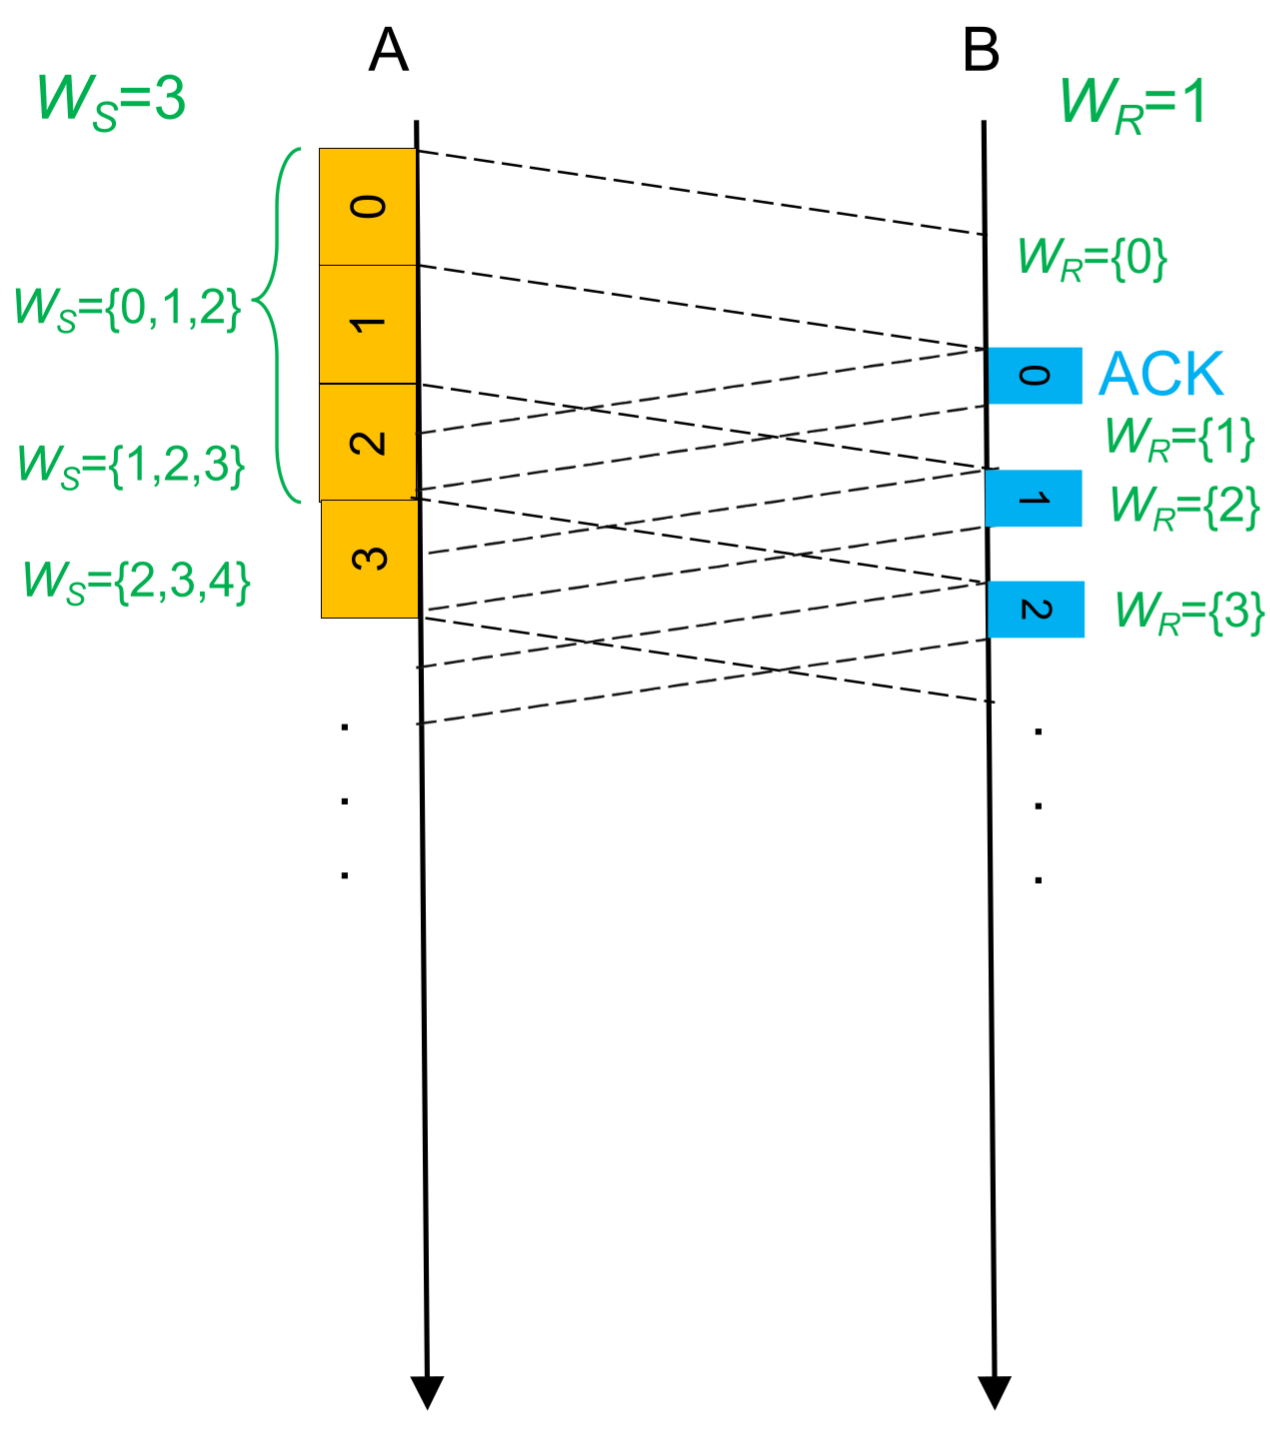
\includegraphics[width=\linewidth]{images/gobackinsenzaerrori.png}
        \caption{Go-Back-N senza errori}
    \end{minipage}%
    \hfill
    \begin{minipage}{0.55\textwidth}
        Nel seguente esempio la finestra di tramissione è 3 e quella di ricezione 1; vengono riscontrati gli ack in modo corretto nei tempi previsti dalla finestra, che nel frattempo ad ogni ack corretto ricevuto scorre di posizione.
        
        Questo vuol dire che nel caso in cui non ci siano errori con l'invio delle trame e con il riscontro degli ack, il seguente protocollo ha efficienza massima.
 
    \end{minipage}
\end{figure}
 \newpage
\subsubsection{Go back N - con errori}
Si possono riscontrare errori durante la ricezione del pacchetto e durante il riscontro degli ack; a seconda della tipologia dell'errore avremo soluzioni differenti.
\paragraph{Errore trasmissione del frame} utilizzo del negative ACK (NACK)
\begin{figure}[htbp]
    \centering
    \begin{minipage}{0.4\textwidth}
        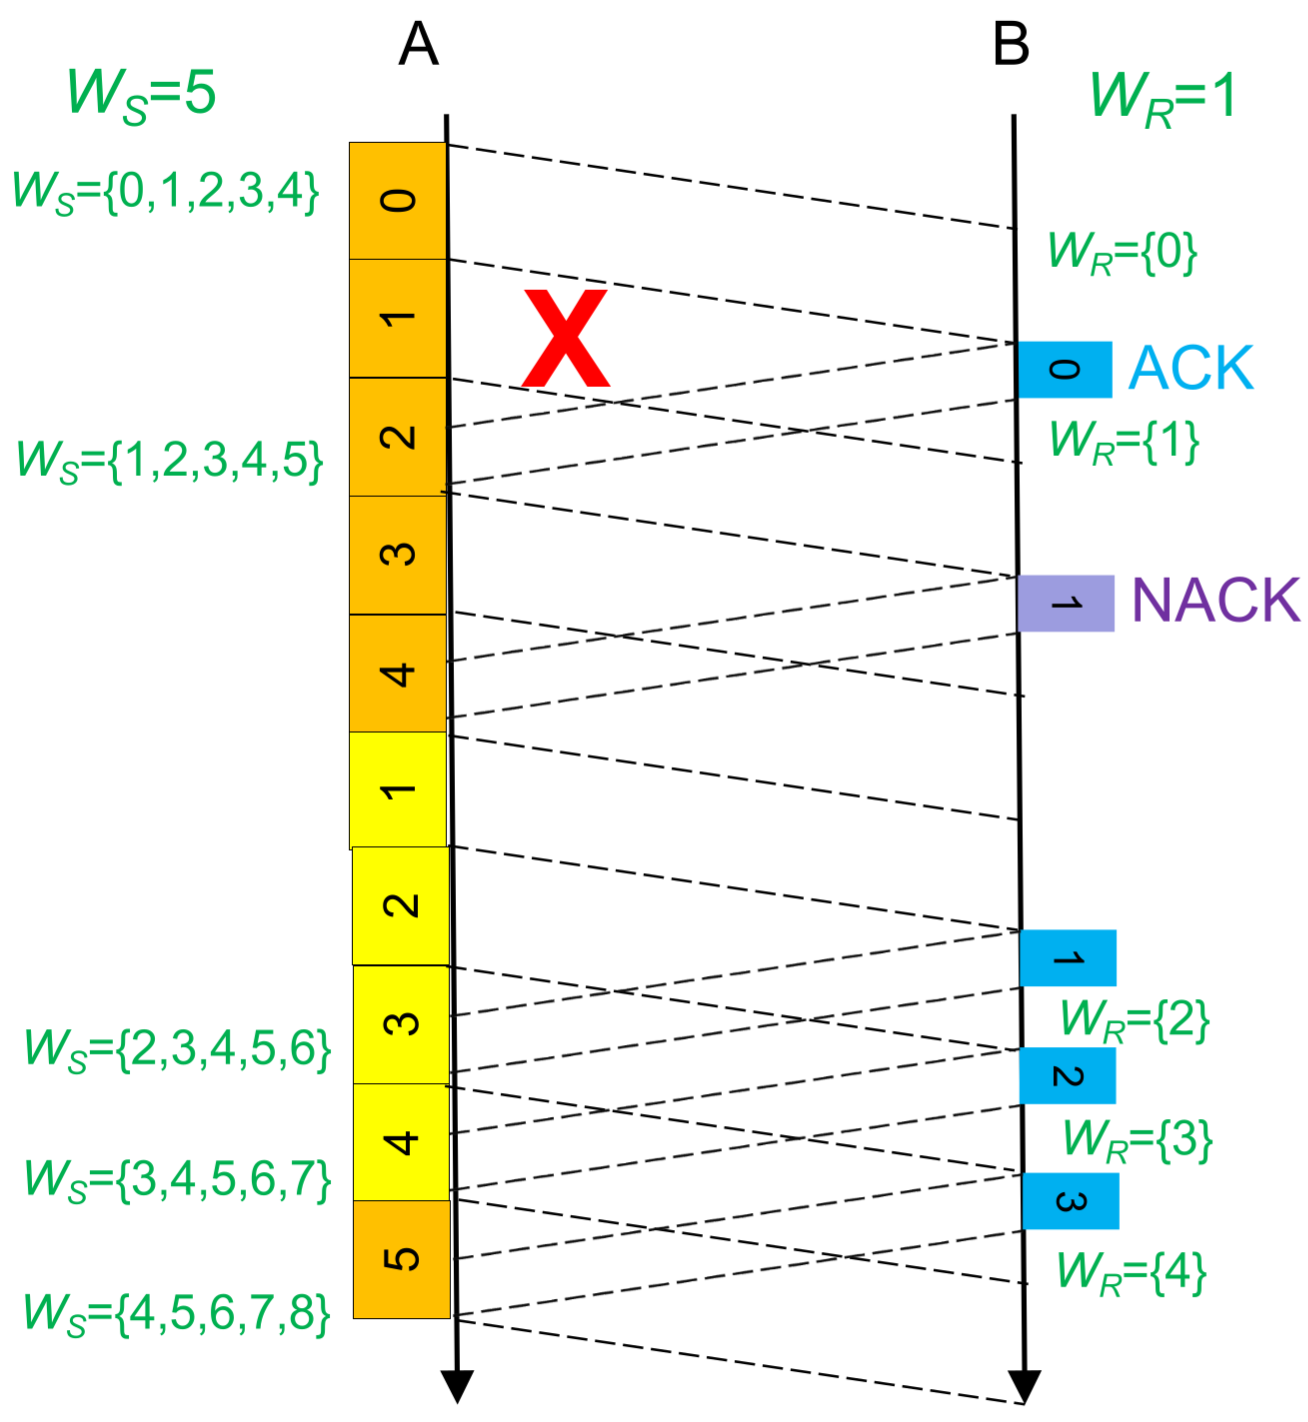
\includegraphics[width=\linewidth]{images/gobackinerrori.png}
        \caption{Go-Back-N con errori in trasmissione}
    \end{minipage}%
    \hfill
    \begin{minipage}{0.55\textwidth}
        Quando si verifica un errore in un frame, il destinatario scarta il frame errato e tutti i frame successivi. 
        
        Il mittente, una volta rilevato l'errore(tramite la ricezione di un NACK(negative ACK) inviato dal destinatario), ritrasmette il frame errato e tutti i frame successivi.
    \end{minipage}
\end{figure}

\paragraph{Errore ACK non ricevuto ($T_{out}$)} caso in cui l'ACK non venga inviato o si sia perso

\begin{figure}[htbp]
    \centering
    \begin{minipage}{0.55\textwidth}
        L'unico modo con il quale il mittente può evitare che il sistema si blocchi in caso di mancato riscontro(neanche NACK),  è quello di avviare un timer ad ogni frame inviato, entro il quale va ricevuto un riscontro.
        
        Se questo timer($T_{out}$) scade allora la finestra torna indietro e ritrasmette da dove è stato riscontrato il problema.
    \end{minipage}%
    \hfill
    \begin{minipage}{0.4\textwidth}
        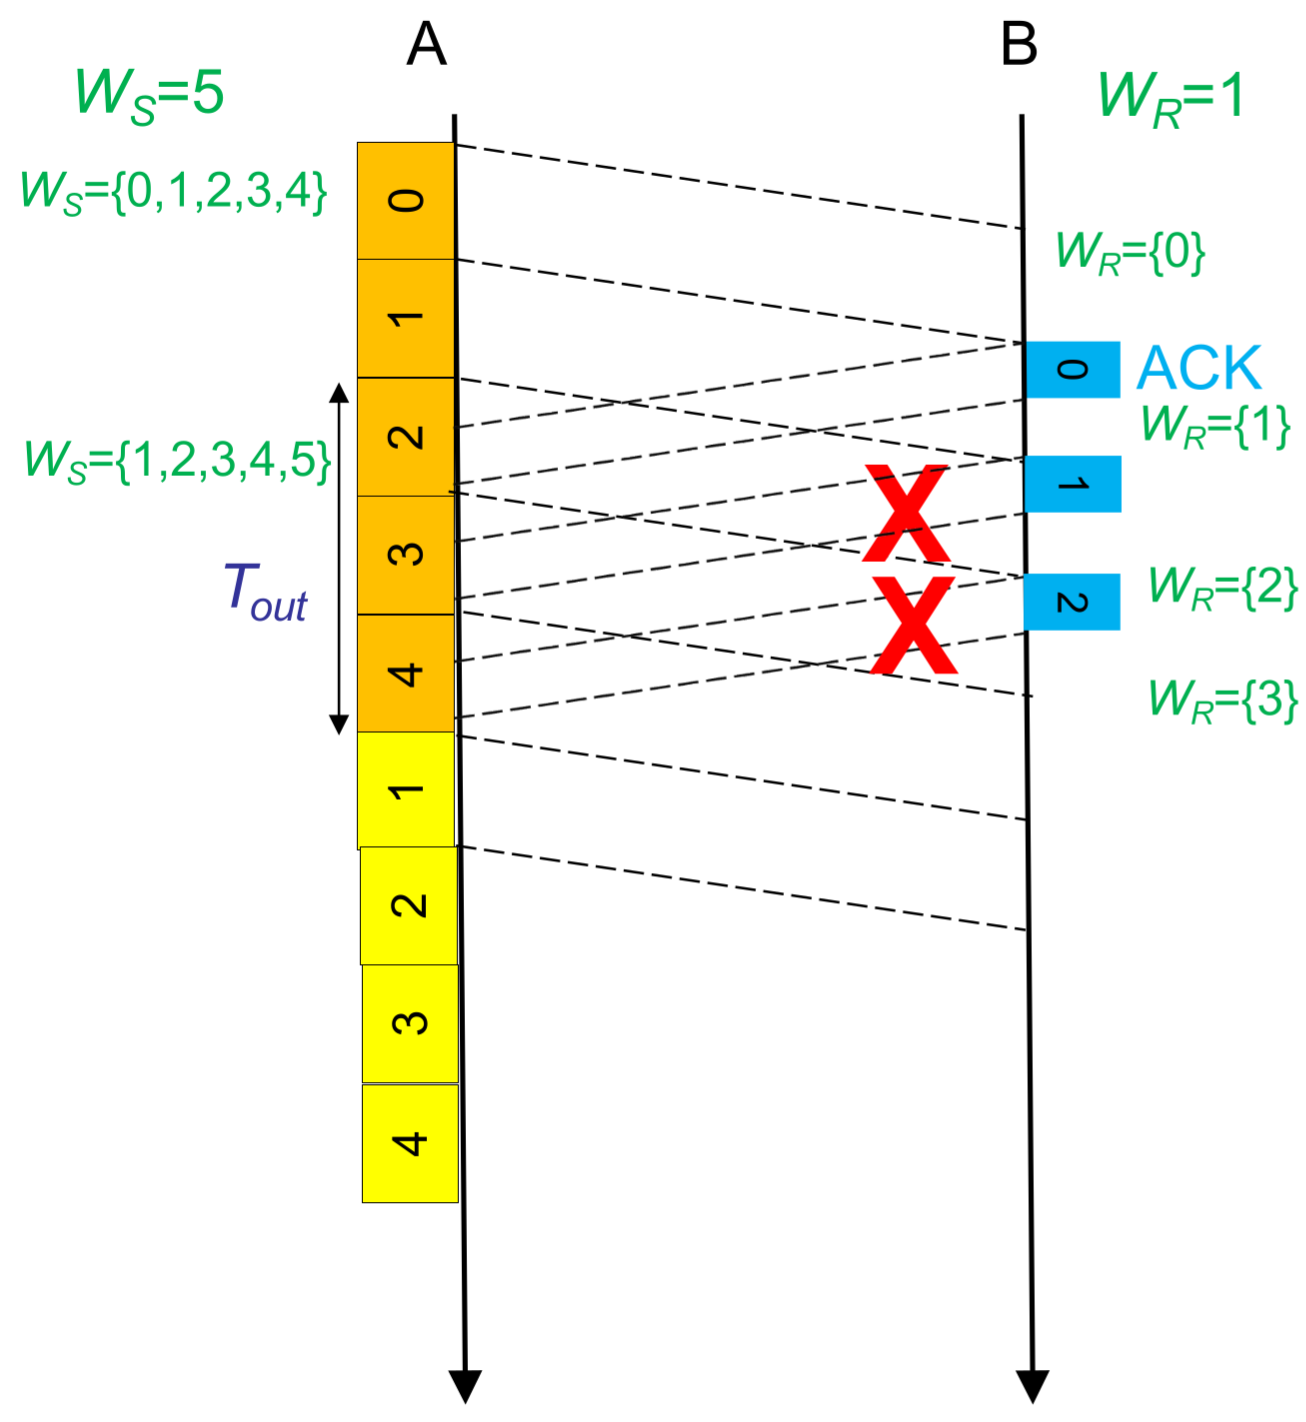
\includegraphics[width=\linewidth]{images/gobacknerroreack.png}
        \caption{Go-Back-N con errore nell'ACK}
    \end{minipage}
\end{figure}


\newpage

\subsubsection{Go back N - ACK equivocato($T_{out}$)} 
con conseguente ricezione di duplicati


\begin{figure}[htbp]
    \centering
    \begin{minipage}{0.5\textwidth}
        \paragraph{Analisi del problema}
        Quando si verifica un equivoco nell'ACK,ossia viene riscontrato erroneamente un frame,  il mittente interpreta erroneamente il riscontro ricevuto e potrebbe ritrasmettere frame già ricevuti correttamente dal destinatario. 
        Questo equivoco può portare a un aumento delle ritrasmissioni e a una riduzione dell'efficienza del protocollo.

L'unico ACK corretto è l'ACK-0, quelli successivi sono errati; nel frattempo la finestra di ricezione ha continuato a scorrere, richiedendo i nuovi 1, 2, etc\dots

Il problema è che i pacchetti 1,2,3 sono già stati ricevuti, l'errore c'è stato solo negli ACK, per i quali il trasmittente sta reinviando 1,2,3 precedenti, che però risulteranno come una copia(il ricevente non lo sa) di quelli trasmessi correttamente prima ma riscontrati in modo errato.

    \end{minipage}%
    \hfill
    \begin{minipage}{0.45\textwidth}
        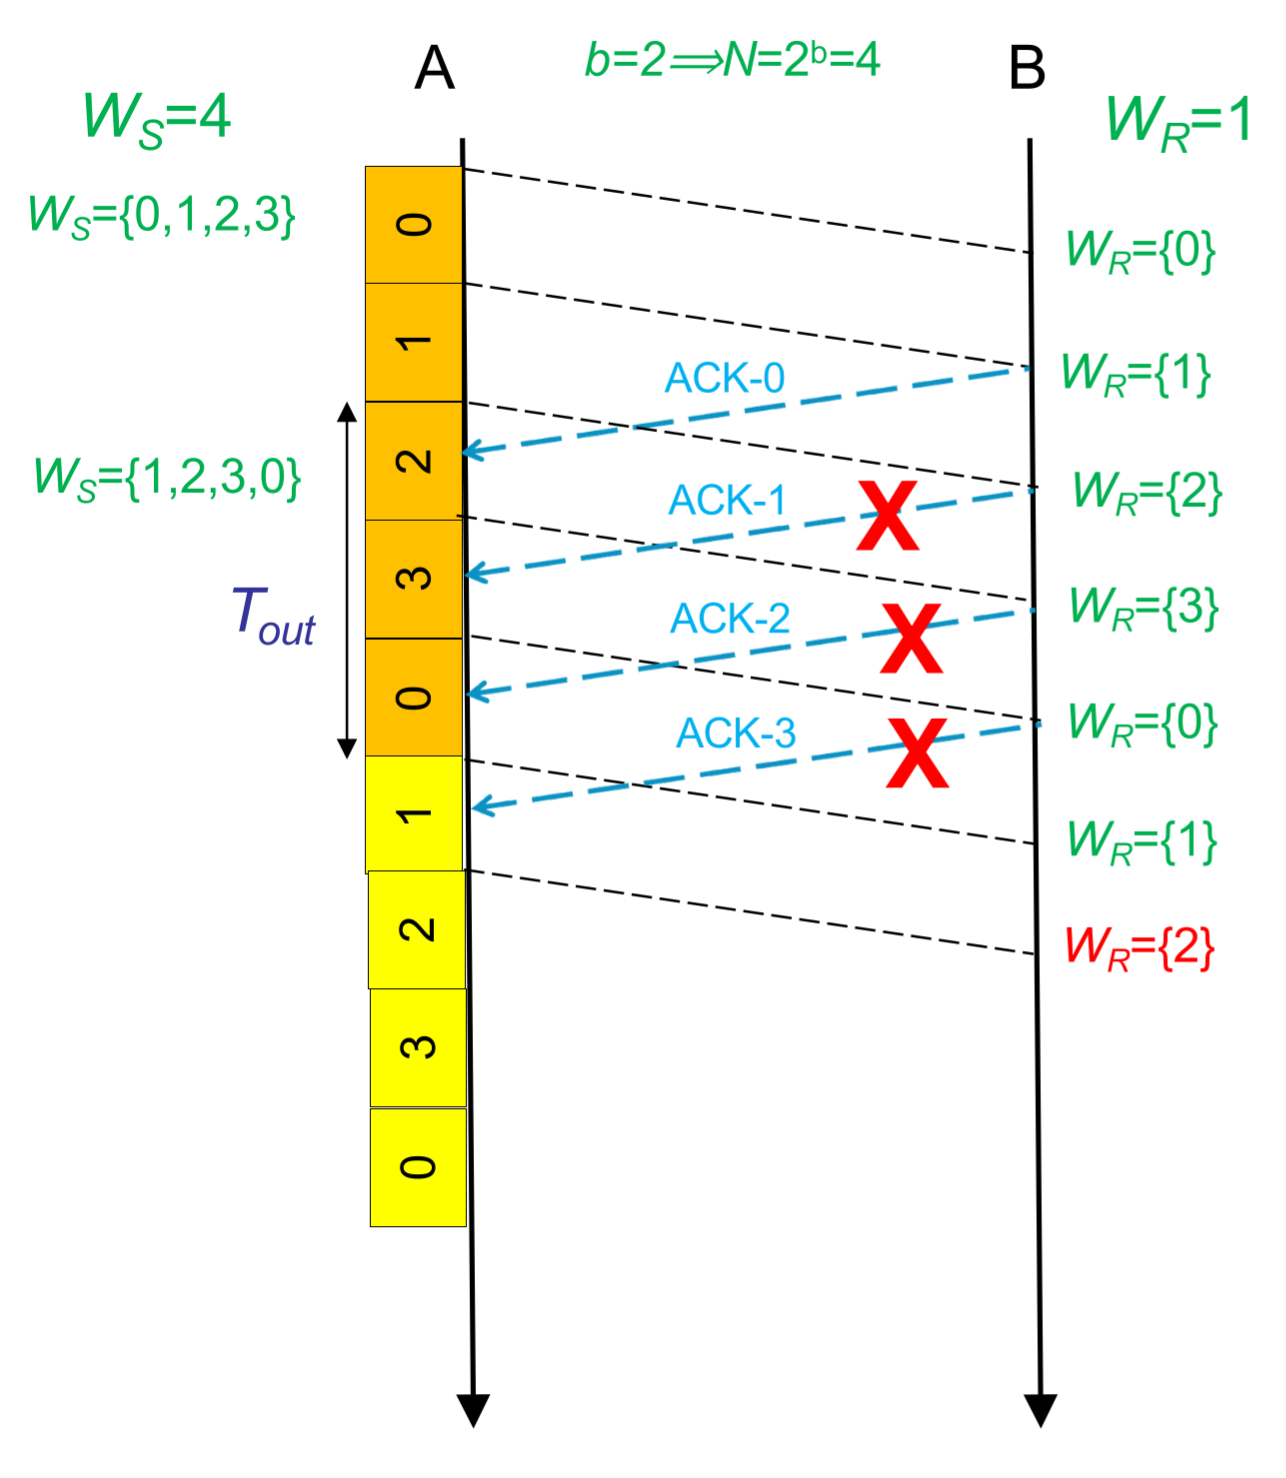
\includegraphics[width=\linewidth]{images/equivocoack.png}
        \caption{Go-Back-N con equivoco nell'ACK}
        
    \end{minipage}
\end{figure}


\begin{figure}[htbp]
    \centering
     \begin{minipage}{0.45\textwidth}
        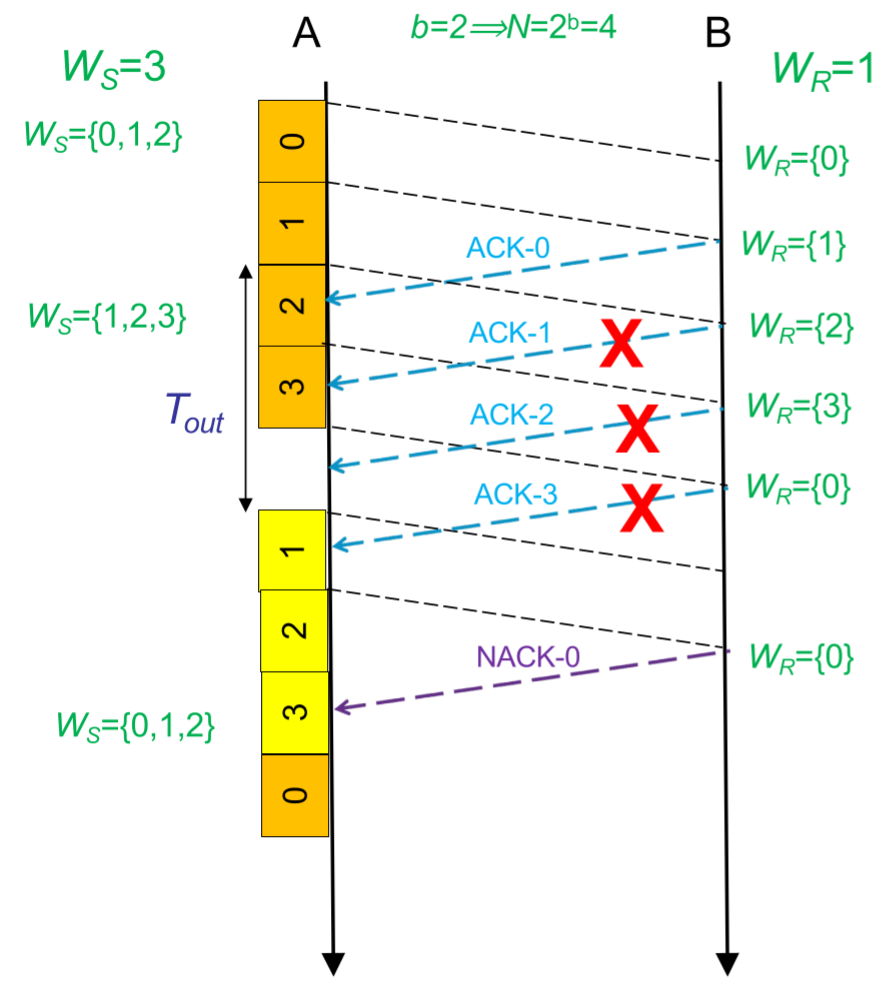
\includegraphics[width=\linewidth]{images/ackequivoco2.png}
        \caption{Go-Back-N con equivoco nell'ACK}

    \end{minipage}
    \hfill
    \begin{minipage}{0.5\textwidth}
        \paragraph{Soluzione} In questo esempio l'unico frame riscontrato correttamente è 0, come nel caso precedente; il problema dei duplicati si risolve poichè il primo frame che non ha avuto un riscontro corretto, ACK-1, ha avviato un timer entro il quale desidera ricevere un riscontro. 
        Al termine di quest'ultimo il trasmettitore ritrasmette dal primo frame che non ha ricevuto riscontro, quindi da 1.

        Il ricevente riceve 1, ma la sua finestra intato ha slideato come se non ci fossero problemi fino a 0; quindi il ricevente si accorge del problema poichè riceve 1 al posto di 0; a questo punto invia un NACK-0 per dire al trasmettitore che quelli ricevuti precedentemente erano corretti, ma riscontrati erroneamnete, quindi desidera continuare la comunicazione dal frame 0, senza ricevere duplicati. ($W_S + W_R \leq N$)

        Questo è possibile perchè la finestra di trasmissione è grande N-1, dove N è il numero di frame.

        
    \end{minipage}%
\end{figure}
\newpage

\subsubsection{Protocollo selective repeat} 
Il protocollo Selective Repeat è un protocollo di tipo Continuous ARQ che consente la ritrasmissione selettiva dei soli frame ricevuti con errore, evitando di ritrasmettere quelli ricevuti correttamente.


        \begin{figure}[htbp]
    \centering
    \begin{minipage}{0.47\textwidth}
        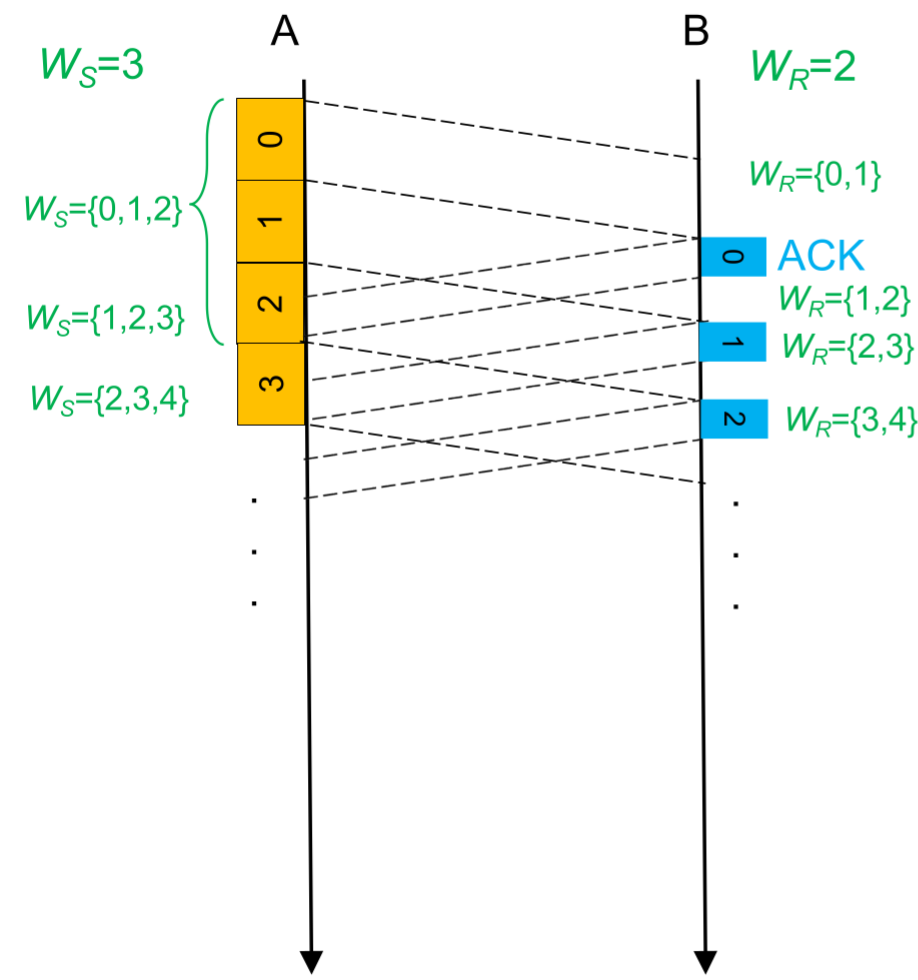
\includegraphics[width=\linewidth]{images/sr.png}
        \caption{Selective Repeat}
        
    \end{minipage}%
    \hfill
    \begin{minipage}{0.48\textwidth}
        \paragraph{In assenza di errori} Questo approccio migliora l'efficienza rispetto al Go-Back-N, poiché la finestra di ricezione può essere maggiore di 1 ($W_R > 1$).

    \end{minipage}
\end{figure}


\begin{figure}[htbp]
    \centering
    \begin{minipage}{0.47\textwidth}
        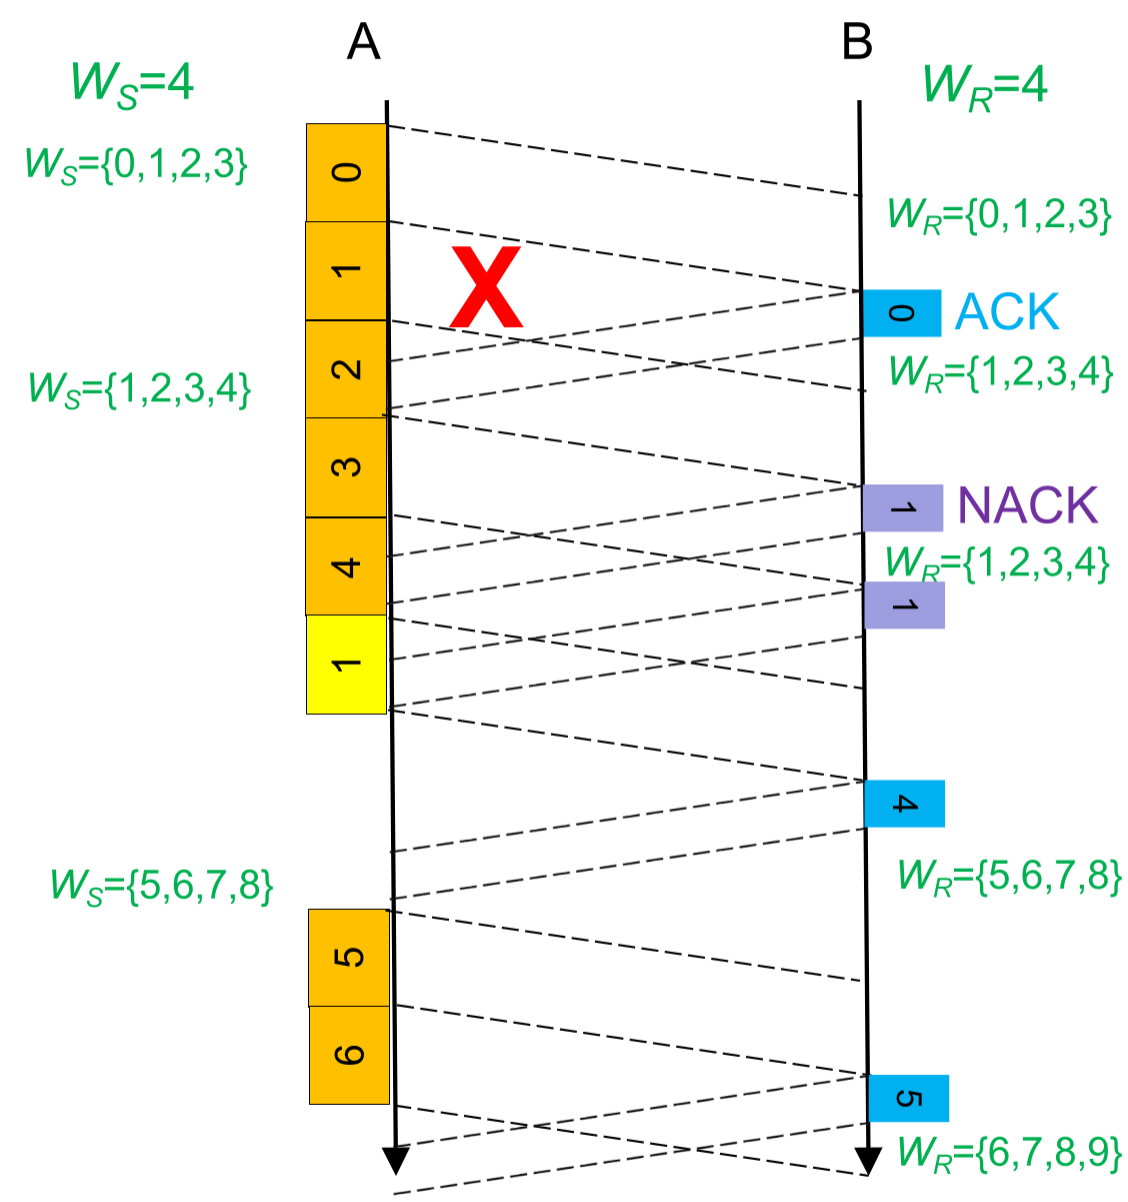
\includegraphics[width=\linewidth]{images/srerroritrama.png}
        \caption{Selective Repeat con errori sulla trama}
    \end{minipage}%
    \hfill
    \begin{minipage}{0.49\textwidth}
        \paragraph{In presenza di errori sul frame}

        Quando si verifica un errore in una trama, il protocollo Selective Repeat consente di ritrasmettere solo la trama errata(il ricevente invia un NACK in cui indica quale frame è andato perso), senza dover ritrasmettere tutte le trame successive come nel Go-Back-N. 

        Questo approccio riduce il numero di ritrasmissioni necessarie e migliora l'efficienza complessiva del protocollo, specialmente in presenza di errori frequenti.
    \end{minipage}
\end{figure}


\newpage

\subsubsection{Selective repeat - equivocazione dei riscontri e soluzione ($T_{out}$)}

\begin{figure}[htbp]
    \centering
    \begin{minipage}{0.48\textwidth}
        \paragraph{Problema equivocazione ACK}
        Il problema sussiste quando i frame vengono trasmessi correttamente, la finestra di ricezione scorre correttamente, ma gli ACK inviati sono errati.

        Perciò come avveniva erroneamente negli altri protocolli, vengono ricevuti dei frame duplicati perchè il trasmettitore riceve degli ACK errati e quindi invia nuovamente i frame rispettivi(alla fine del $T_{out}$) a questi ACK; ma questi frame risulteranno a tutti gli effetti dei duplicati di quelli ricevuti correttamente dal ricevitore.
    \end{minipage}%
    \hfill
    \begin{minipage}{0.45\textwidth}
        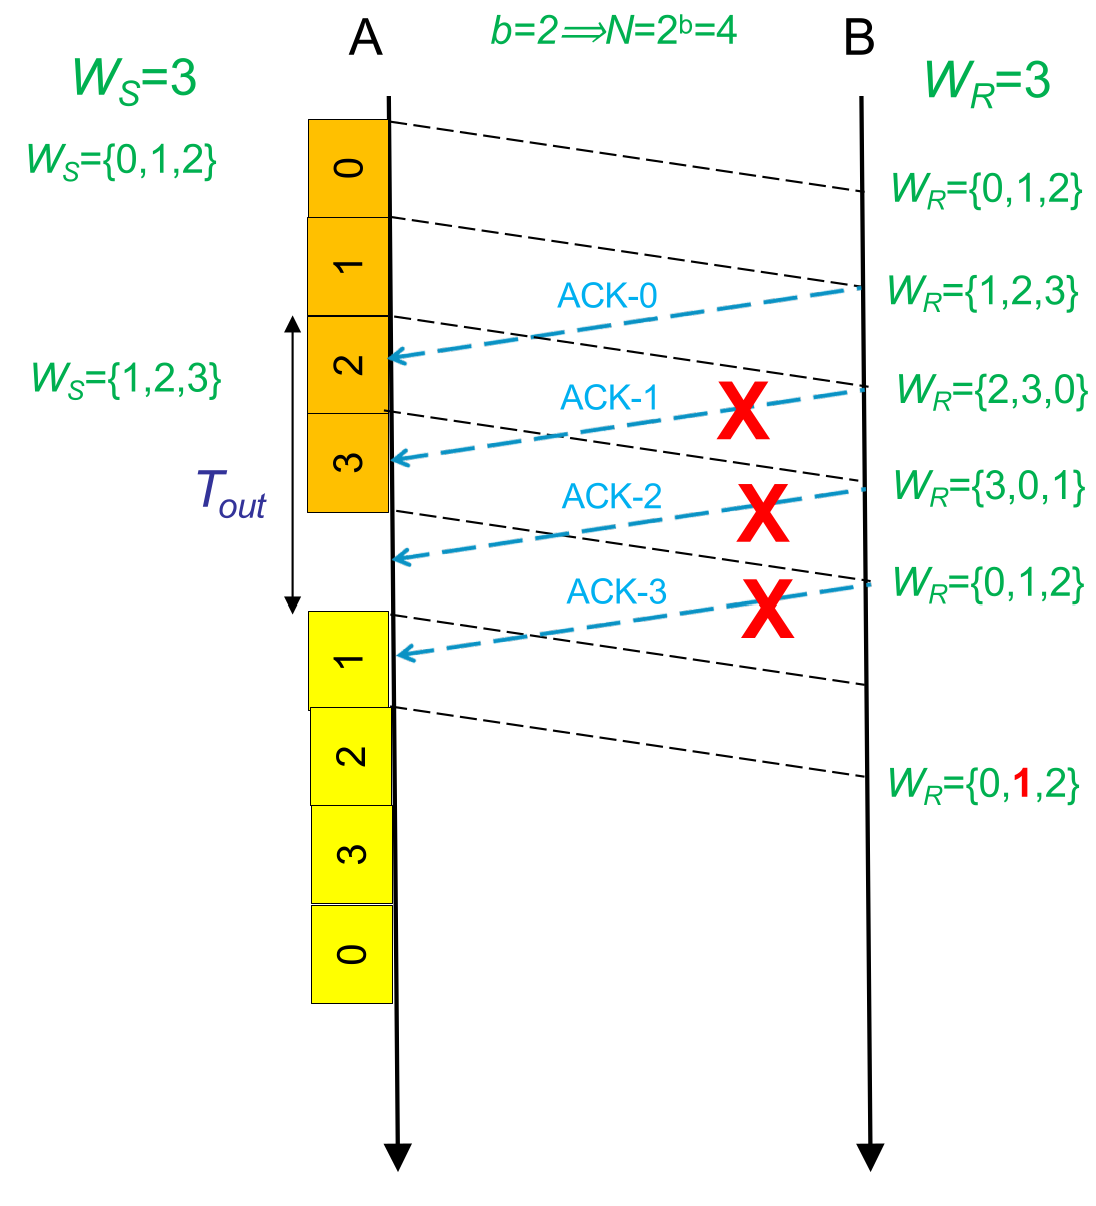
\includegraphics[width=\linewidth]{images/srequivocazione.png}
        \caption{Selective Repeat con errori sull'ACK}
    \end{minipage}
\end{figure}


\begin{figure}[htbp]
    \centering
    \begin{minipage}{0.48\textwidth}
        \paragraph{Soluzione}
        Questo problema viene risolto diminuendo la grandezza delle finestre($W_S + W_R \leq N$), secondo i criteri discussi nel capoverso successivo.
    \end{minipage}%
    \hfill
    \begin{minipage}{0.435\textwidth}
        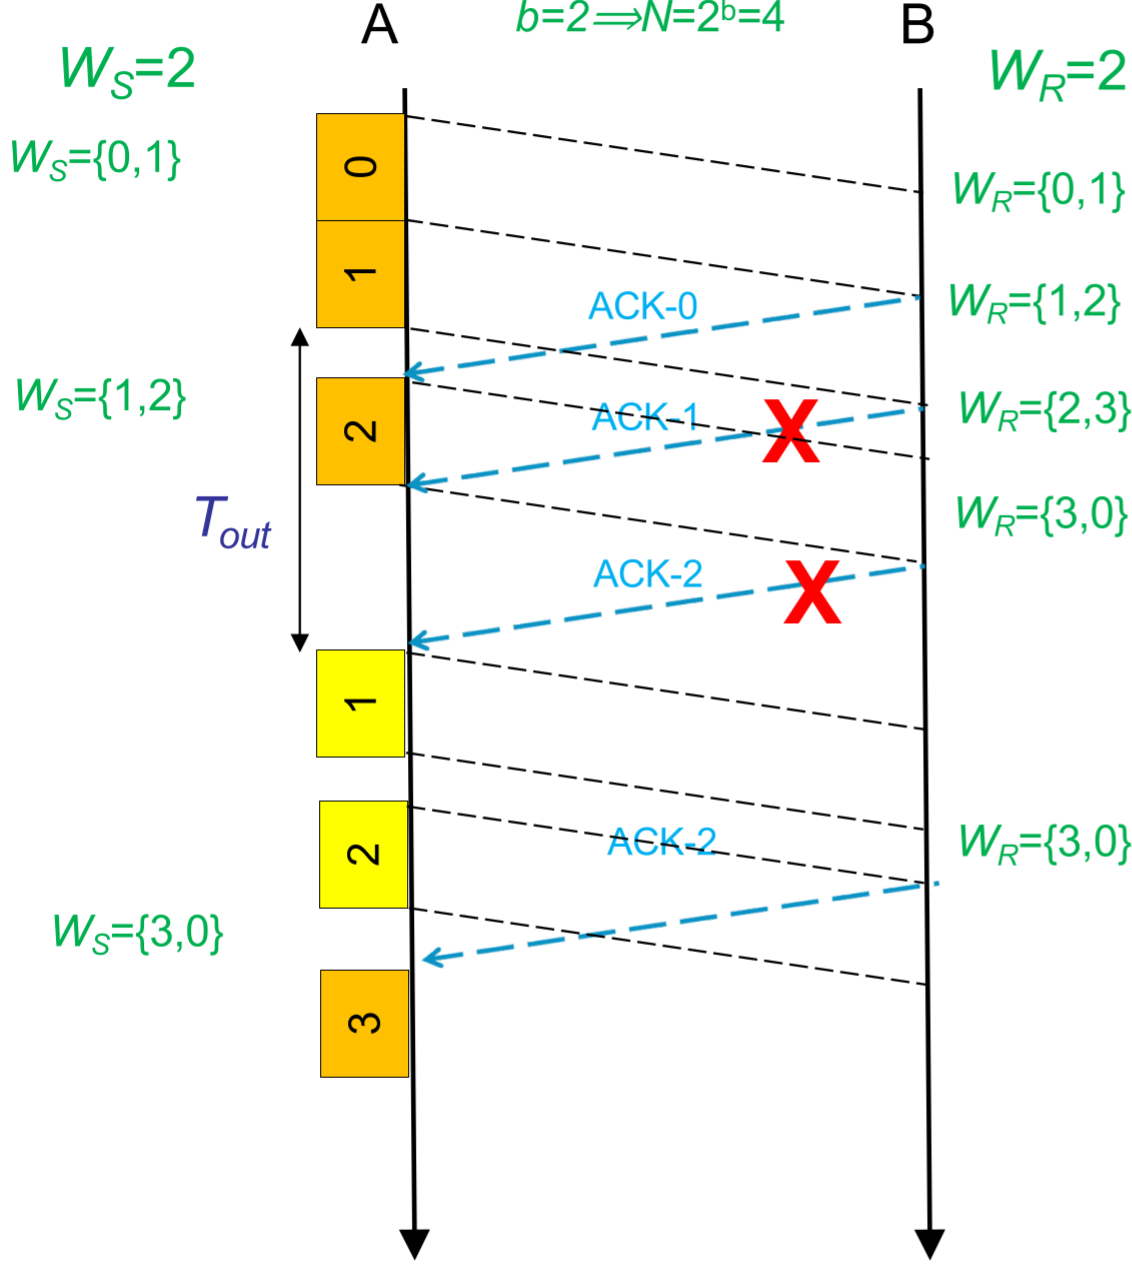
\includegraphics[width=\linewidth]{images/equivocazionesr.png}
        \caption{Selective Repeat con equivocazione risolta}
    \end{minipage}
\end{figure}

\newpage

\subsection{Dimensione delle finestre di trasmissione/ricezione}
Con la visione degli esempi riguardanti l'equivocazione, si può affermare che in entrambi i protocolli continous ARQ, Go-Back-N e Selective Repeat, le finestre di trasmissione e di ricezione non possono essere pari a o maggiori di N in quanto si avrebbe equivocazione:

\begin{center}
\begin{minipage}{0.45\textwidth}
    \begin{equation*}
        \begin{cases}
            W_S \leq N \\
            W_R \leq N
        \end{cases}
    \end{equation*}
\end{minipage}
\hfill
\begin{minipage}{0.45\textwidth}
    \begin{equation*}
        W_S + W_R \leq N
    \end{equation*}
\end{minipage}
\end{center}
Inoltre le finestre non devono sovrapporsi, poichè in caso di equivoco e di scorrimento completo della finestra di ricezione, si potrebbe riscontrare il problema di ricezione di duplicati; anche questo si risolve imponendo una condizione sulla grandezza di tali finestre:

\subsubsection{Dimensione finestre GBN ed efficienza massima}

\begin{minipage}{0.55\textwidth}
Nel caso di GBN, la finestra di ricezione è necessariamente
unitaria. Per cui la finestra di trasmissione deve essere al più
N-1; poiché non conviene fissarla ad un valore inferiore al
massimo (riduzione del throughput non giustificata), la scelta
ottimale è fissare: 
\end{minipage}%
\hfill
\begin{minipage}{0.4\textwidth}
\begin{equation*}
    \begin{cases}
        W_S = N-1 \\
        W_R = 1
    \end{cases}
\end{equation*}
\end{minipage}

\subsubsection{Dimensione finestre SR ed efficienza massima}
Nel caso del selective repeat vanno considerati più fattori:

\begin{itemize}
    \item non ha senso scegliere la finestra di
trasmissione maggiore di quella di ricezione, perché si
trasmetterebbero più trame di quante ne può ricevere e
ordinare il ricevente
    \item  non ha senso scegliere la finestra di
ricezione maggiore di quella di trasmissione perché si
ridurrebbe il throughput trasmettendo meno trame di quelle
che si possono ricevere
\end{itemize}
Pertanto la soluzione ottimale è: $W_S = W_R = \frac{N}{2}$
\subsection{Effcienza GBN $\&$ SR}
\begin{figure}[htbp]
    \centering
    \begin{minipage}{0.4\textwidth}
        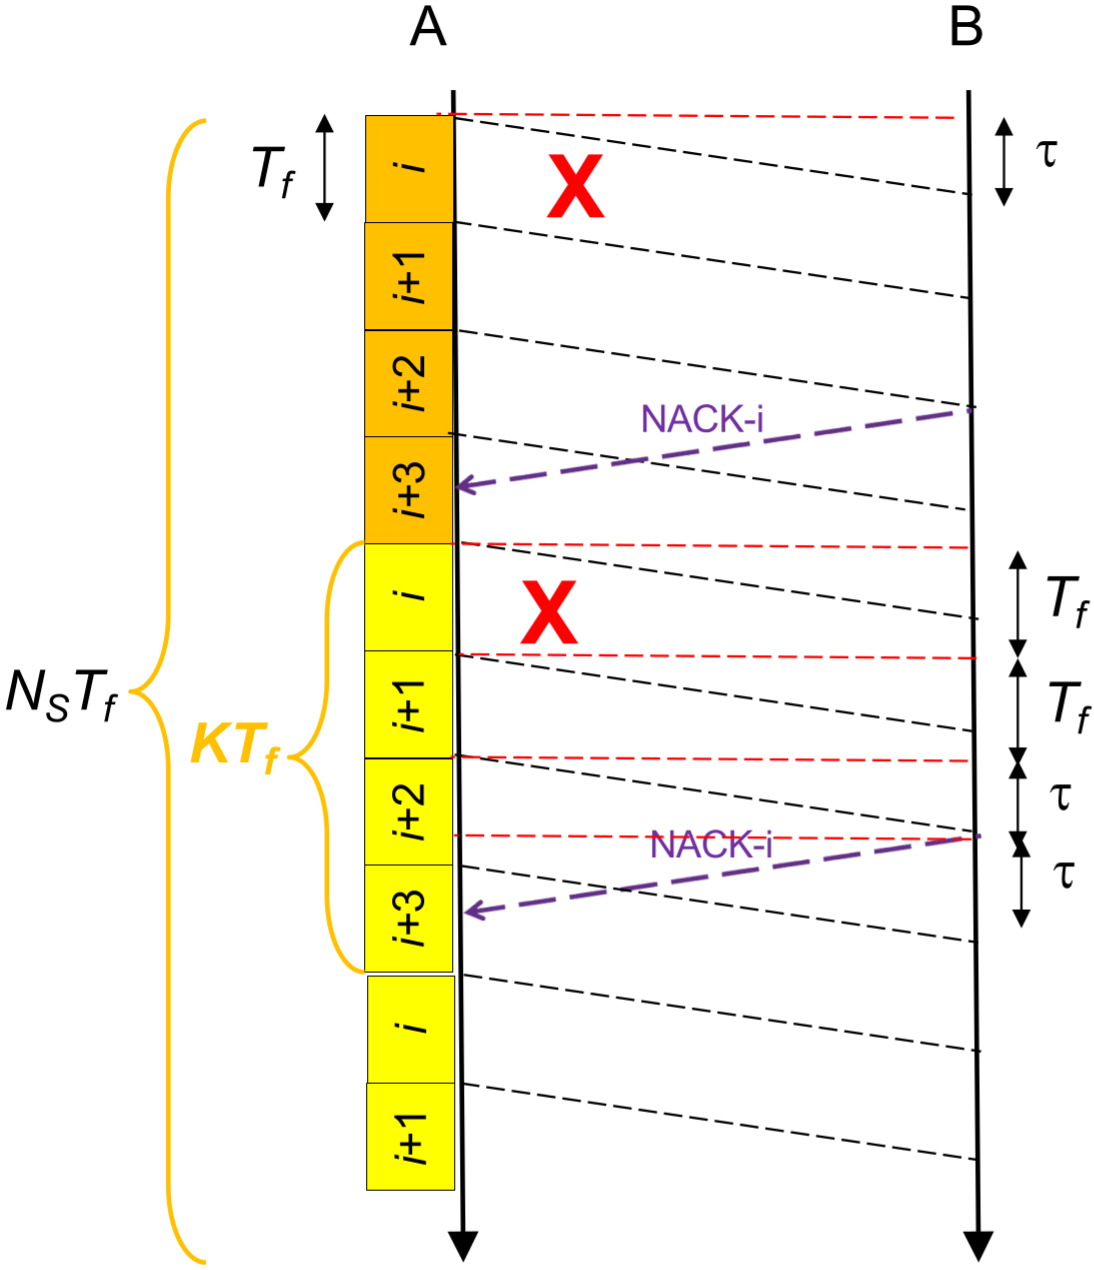
\includegraphics[width=\linewidth]{images/efficienzagbn.png}
        \caption{Efficienza del protocollo Go-Back-N}
    \end{minipage}%
    \hfill
    \begin{minipage}{0.5\textwidth}
        \paragraph{Efficienza Go-Back-N}
        Il trasmettitore si accorge dell'errore sulla trama i solo dopo i+x, dove x dipende dalla finestra di trasmissione e dal tempo in cui impiega ad arrivare il NACK-i relativo al frame errato.

        Il costo della trasmissione del frame corretto è $N_ST_f$, dove $N_S$ è il numero di frame che sono stati trasmessi e ritrasmessi per la corretta trasmissione di quel frame, pari a:
        \begin{equation}
        N_S = ("numero\_errori" * K) + 1
        \end{equation}

        K è il numero di trame che vengono ritrasmesse ad ogni errore, il + 1 il frame corretto.

    \end{minipage}
\end{figure}

Considerando il valore medio delle trame trasmesse in totale, $N_S$, il tempo totale equivale a:
        
        \begin{equation}
        T_{tot} = \overline{N_S} * T_f 
        \end{equation}
        
        da cui l'efficienza $\eta$ è pari al reciproco di $\overline{N_S}$:

        \begin{equation}
        \eta = \frac{T_f}{\overline{N_S} \cdot T_f} = \frac{1}{\overline{N_S}}
        \end{equation}

        \begin{figure}[htbp]
            \centering
            \begin{minipage}{0.4\textwidth}
                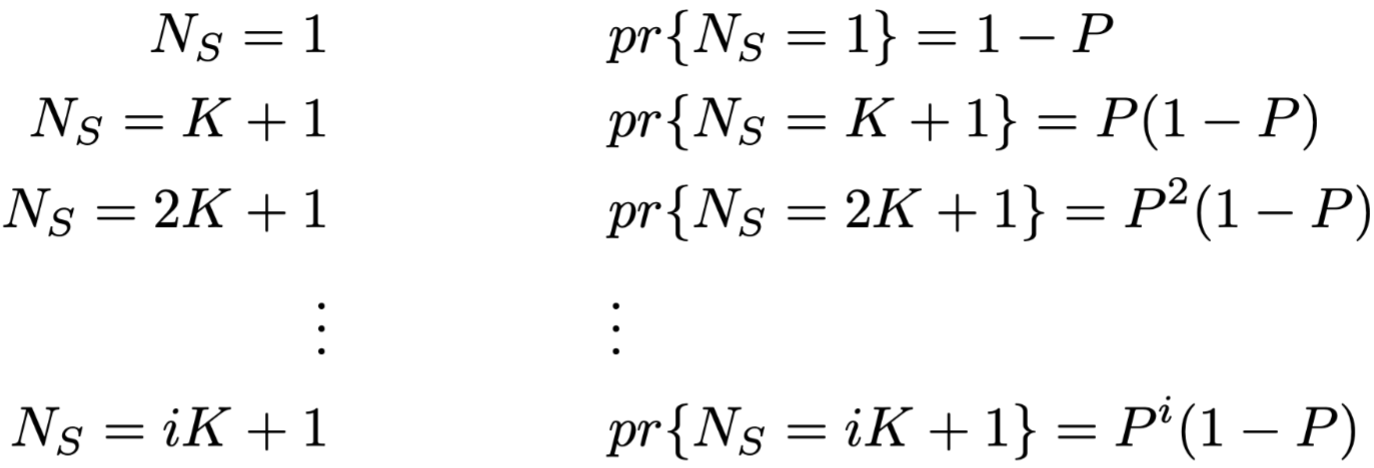
\includegraphics[width=\linewidth]{images/gbnns.png}
                \caption{Calcolo probabilità di $N_S$}
            \end{minipage}%
            \hfill
            \begin{minipage}{0.55\textwidth}
                Nella prima riga si illustra il caso in cui non ci siano errori, per cui $numero_{errori}*K + 1$ vale 1;

                nel secondo rigo l'errore è uno, nel terzo rigo gli errori sono due$(numero_{errori} = 2)$ e così via, fino al calcolo generale di $N_S = iK + 1$

                Inoltre si calcola la probabilità pr 
            \end{minipage}
        \end{figure}
\paragraph{Calcolo del valor medio di $N_S$}

Il valor medio si otterrà sommando i valori assunti dalla variabile "i" per la probabilità di assumerli:

\begin{equation*}
\overline{N_S} = E[N_S] = \sum_{i=0}^{+\infty} (iK + 1) P^i (1-P) = (1-P) \left[ \sum_{i=0}^{+\infty} iK P^i + \sum_{i=0}^{+\infty} P^i \right] =
\end{equation*}
\begin{equation*}
(1-P) \left[ KP \sum_{i=1}^{+\infty} i P^{i-1} + \frac{1}{1-P} \right] = (1-P) \left[ \frac{KP}{(1-P)^2} + \frac{1}{1-P} \right] = \frac{1 + P(K-1)}{1-P}
\end{equation*}

\subsubsection{Quanto vale K}
Dal grafico sull'efficienza si può individuare il valore di K approssimato:

\begin{equation}
KT_f \simeq 2T_f + 2\tau \implies K = 2 + 2\alpha
\end{equation}

sostituendo K nella formula dell'efficienza ottengo:

\begin{equation}
\eta = \frac{1-P}{1 + P(K-1)} = \frac{1-P}{1 + P(1 + 2\alpha)}
\end{equation}


\newpage


\subsection{Efficienza GBN $\&$ SR}
\begin{figure}[htbp]
    \centering
    \begin{minipage}{0.4\textwidth}
        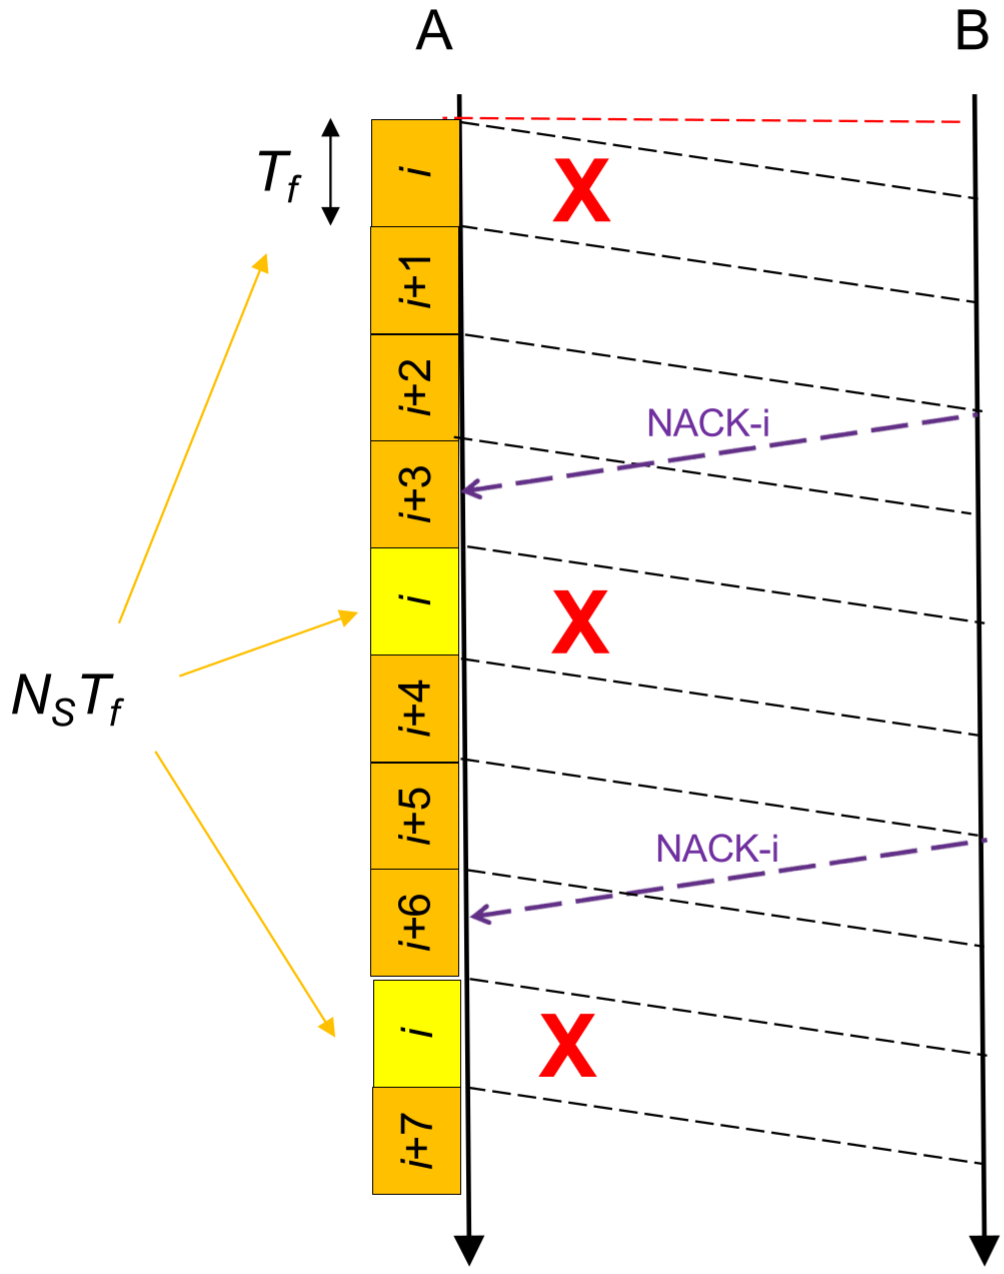
\includegraphics[width=\linewidth]{images/efficienzasr.png}
        \caption{Efficienza del protocollo Selective Repeat}
    \end{minipage}%
    \hfill
    \begin{minipage}{0.55\textwidth}
        \paragraph{Efficienza Selective Repeat}
        Nel protocollo Selective Repeat, grazie alla ritrasmissione selettiva dei soli frame errati, l'efficienza risulta superiore rispetto al Go-Back-N, soprattutto in presenza di errori frequenti. 

        Per valutarne l'efficienza si suppone che:
        \begin{itemize}
            \item i riscontri arrivino all'interno della finestra di trasmissione
            \item l'eventuale trama sbagliata sia sempre la stessa
            \item si trascurano i tempi di elaborazione e di trasmissione degli ack($\tau, T_P$)
        \end{itemize}

        l'efficienza la calcoliamo allo stesso modo:

        \begin{equation}
        \eta = \frac{T_f}{T_{tot}}
        \end{equation}
         \begin{equation}
        \eta = \frac{T_f}{\overline{N_S} \cdot T_f} = \frac{1}{\overline{N_S}}
        \end{equation}

        va capito quanto vale $T_{tot}$

    \end{minipage}
\end{figure}

Per calcolare $T_{tot}$ ho bisogno di individuare il valore medio di $N_S$:

\begin{figure}[htbp]
    \centering
    \begin{minipage}{0.45\textwidth}
        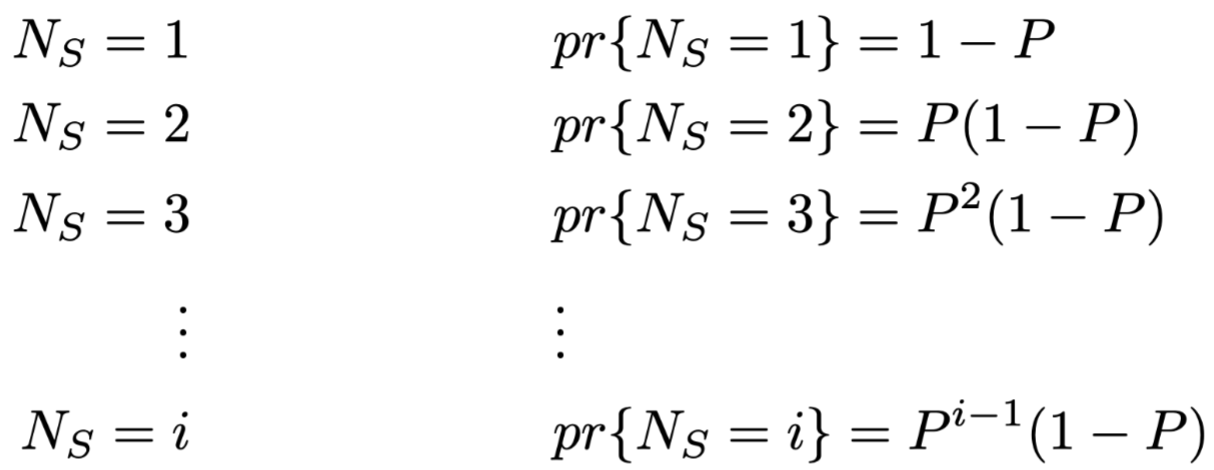
\includegraphics[width=\linewidth]{images/nssr.png}
        \caption{Calcolo del valor medio di $N_S$ per Selective Repeat}
    \end{minipage}%
    \hfill
    \begin{minipage}{0.5\textwidth}
        Nel protocollo Selective Repeat, il valore medio di $N_S$ (numero di trasmissioni per frame corretto) si calcola considerando che ad ogni errore viene ritrasmesso solo il frame errato. La variabile aleatoria $N_S$ segue una distribuzione geometrica come nel caso Stop-and-Wait, quindi:
        \[
        \overline{N_S} = E[N_S] = \sum_{i=1}^{+\infty} i P^{i-1}(1-P) = \frac{1}{1-P}
        \]
        dove $P$ è la probabilità di errore sul frame. L'efficienza risulta quindi:
        \[
        \eta = 1 - P
        \]
    \end{minipage}
\end{figure}

Si vede chiaramente che il SR ha l'efficienza più elevata tra
tutti i protocolli di linea, ma è quello con la maggiore
complessità (e quindi costi più alti) per la presenza dei due
buffer (in trasmissione e ricezione) e per la necessità di
gestire il riordinamento.

\begin{center}
\begin{minipage}{0.45\textwidth}
    \textbf{Go-Back-N}
    \begin{equation*}
        \eta_{GBN} = \frac{1-P}{1 + P(1 + 2\alpha)}
    \end{equation*}
\end{minipage}
\hfill
\begin{minipage}{0.45\textwidth}
    \textbf{Selective Repeat}
    \begin{equation*}
        \eta_{SR} = 1 - P
    \end{equation*}
\end{minipage}
\end{center}

Quando nel caso ideale non si considerano gli errori (P=0),
GBN e SR hanno stessa efficienza pari a 1 (la massima
teorica).

Si noti però che per valori piccoli del ritardo di
propagazione normalizzato a tutti i protocolli hanno
efficienza comparabile e pari a 1-P per cui, in tal caso,
sono equivalenti.

\newpage

\subsection{Efficienza con riscontri fuori dalla finestra di trasmissione $W_s$}

\begin{figure}[htbp]
    \centering
    \begin{minipage}{0.45\textwidth}
        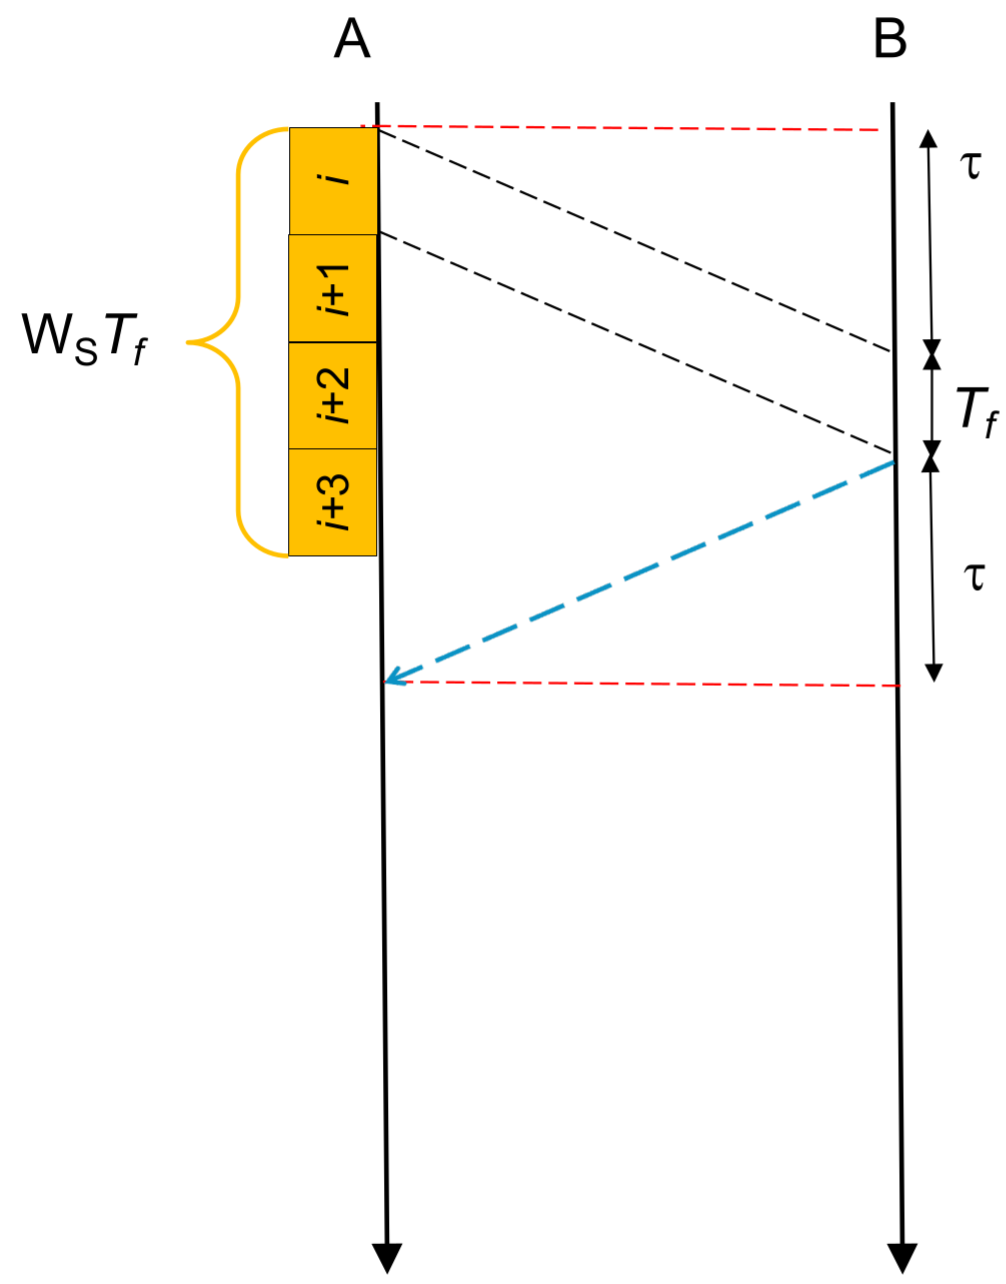
\includegraphics[width=\linewidth]{images/efficienzasrwr.png}
        \caption{Riscontri fuori dalla finestra di trasm. $W_s$}
    \end{minipage}%
    \hfill
    \begin{minipage}{0.5\textwidth}
        Fino ad ora ho studiato l'efficienza di questi protocolli nel caso in cui i riscontri arrivino all'interno della finestra di trasmissione; se però ciò non accade, quindi i riscontri arrivano fuori dalla finestra, l'efficienza sarà inferiore.

        Il tempo che impiega A a trasmettere tutti i frame delle finestra è necessariamente minore del tempo che impiega il primo frame a raggiungere B e ad essere processato(da cui calcolo la finestra):

        \begin{equation}
        W_S T_f \leq T_f + 2\tau \implies W_S \leq 1 + 2\alpha
        \end{equation}

            Il primo ACK arriverà al di fuori di questa finestra, quindi impiegherà almeno $T_f + 2\tau$

    \end{minipage}

\end{figure}

Pertanto l'efficienza degli schemi visti prima, va moltiplicata
per un fattore(w) di efficienza che pesa l'efficienza finale e che
rappresenta il valore limite per SR e GBN nel caso di
assenza di errori e riscontri fuori dalla finestra di
trasmissione. Tale valore è dato dal rapporto tra tempo utile
di occupazione del canale e tempo di attesa del primo
riscontro:

\begin{equation}
\eta_W = \frac{W_S T_f}{T_f + 2\tau} = \frac{W_S}{1 + 2\alpha}
\end{equation}

Per cui le efficienze si SR e GBN sono:

\begin{center}
\begin{minipage}{0.45\textwidth}
    \begin{equation*}
        \eta_{GBN} = \frac{1-P}{1 + P(W_S - 1)} \cdot \frac{W_S}{1 + 2\alpha}
    \end{equation*}
\end{minipage}
\hfill
\begin{minipage}{0.45\textwidth}
    \begin{equation*}
        \eta_{SR} = (1-P) \cdot \frac{W_S}{1 + 2\alpha}
    \end{equation*}
\end{minipage}
\end{center}
Nel GBN invece, il valore K è proprio $W_S$ in quanto in caso di errore si ritrasmette l'intera finestra.
Se si ipotizza stesso valore di $N$ per SR e GBN, considerando il valore ottimale delle finestre, si ha:

\begin{align*}
    \eta_{GBN} &= \frac{1-P}{1 + P(N-2)} \cdot \frac{N-1}{1 + 2\alpha} \\
    \eta_{SR}  &= (1-P) \cdot \frac{N/2}{1 + 2\alpha}
\end{align*}

\newpage

\subsection{Confronto tra protocolli di linea}
\paragraph{Confronto tra protocolli}

\begin{figure}[htbp]
    \centering
    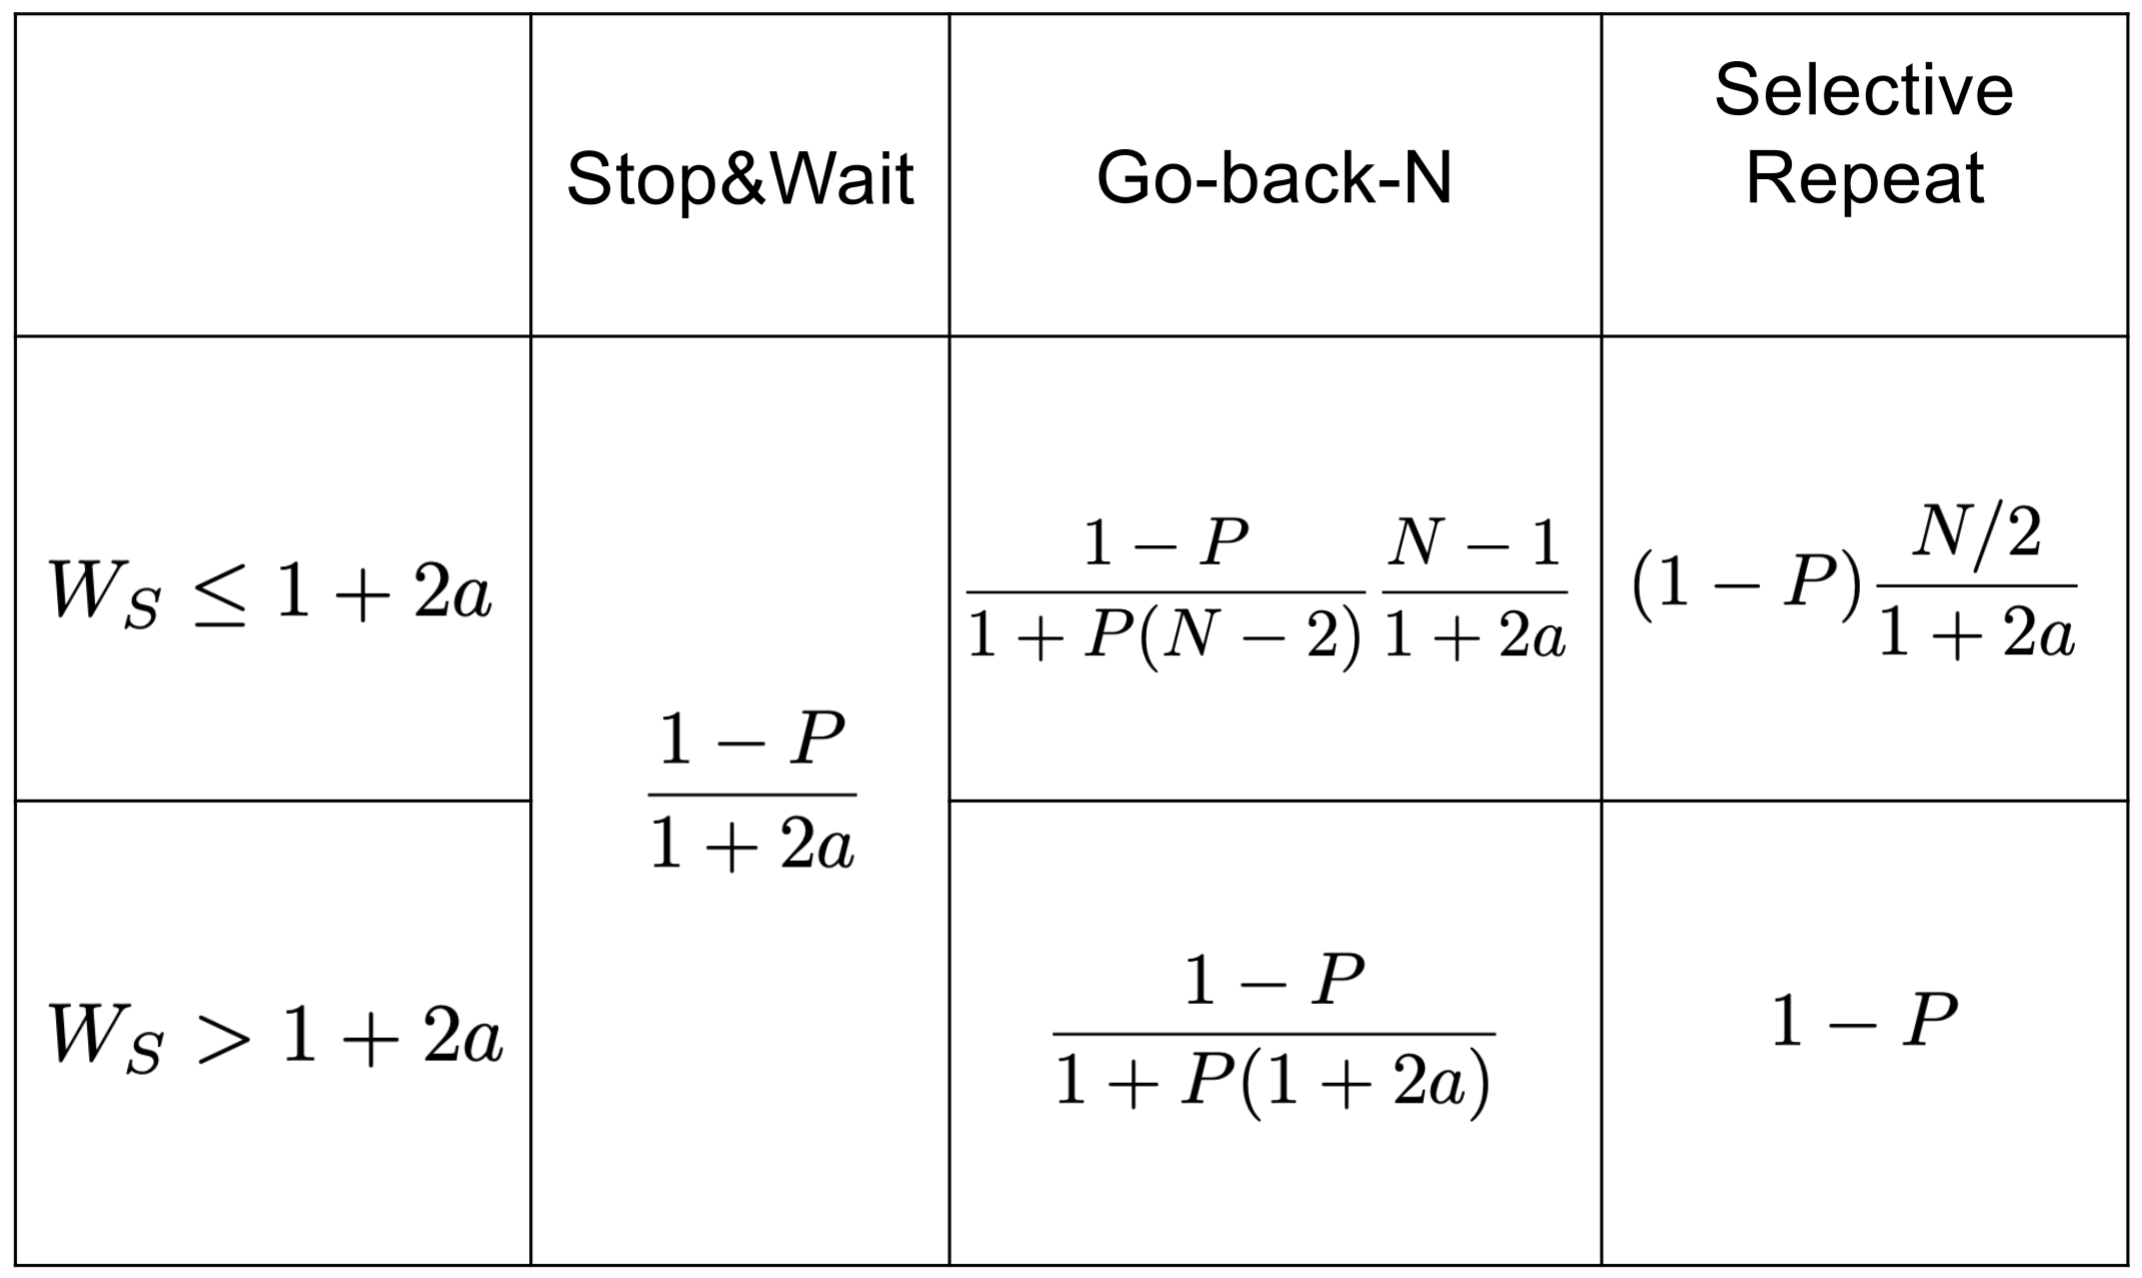
\includegraphics[width=0.7\textwidth]{images/confrontoprotocolli.png}
    \caption{Confronto dell'efficienza tra i protocolli Stop-and-Wait, Go-Back-N e Selective Repeat}
\end{figure}

        Il grafico mostra l'andamento dell'efficienza dei protocolli Stop-and-Wait, Go-Back-N e Selective Repeat al variare del ritardo di propagazione normalizzato $\alpha$ e della probabilità di errore $P$.\\
        La scelta del protocollo di linea dipende dalla situazione:
        \begin{itemize}
            \item caso in cui i riscontri siano all'interno della finestra di ricezione: SR è sempre più efficiente, ma per bassi valori di $\alpha$ tutti hanno efficienza simile e pari a 1-P
            \item caso in cui i riscontri siano fuori della finestra di trasmissione: il diverso valore della finestra di trasmissione può
rendere più efficiente GBN rispetto al SR, 
            \item canali poco rumorosi(P basso) e $\alpha$ elevato: si
può avere un'efficienza maggiore del GBN: infatti, è vero che
con il GBN si ritrasmette l'intera finestra, ma questo evento
accade raramente, mentre durante la trasmissione senza errori
si trasmettono più frame di continuo (es. link satellitari) 
            \item canali molto rumorosi(P alto): sarà nuovamente più
efficiente il SR poiché si ritrasmette spesso per cui conviene
ritrasmettere la singola trama piuttosto che l'intera finestra
        \end{itemize}
        La scelta del protocollo dipende dal compromesso tra efficienza, complessità($\$$) e condizioni del canale.

        